\chapterhead{CHƯƠNG 4 $-$ TRIỂN KHAI, CẤU HÌNH VPN}
\addcontentsline{toc}{chapter}{CHƯƠNG 4 $-$ TRIỂN KHAI, CẤU HÌNH VPN}
\vspace{-0.5cm}
\section*{4.1 Triển khai VPN trên Windows Server (GUI)}
 \addcontentsline{toc}{section}{4.1 Triển khai VPN trên Windows Server (GUI)}


 \subsection*{4.1.1 Xây dựng Remote Access VPN}
 \addcontentsline{toc}{subsection}{4.1.1 Xây dựng Remote Access VPN}

\subsubsection*{4.1.1.1 Chuẩn bị thiết bị}
 \addcontentsline{toc}{subsubsection}{4.1.1.1 Chuẩn bị thiết bị}

 \begin{itemize}
     \item Một máy chủ WindowServer làm VPN Server.
     \item Một máy Client1 làm người dùng client ở ngoài Internet có thể truy cập vào mạng doanh nghiệp để lấy tài liệu làm việc.
 \end{itemize}

\subsubsection*{4.1.1.2 Thực hiện cấu hình}
 \addcontentsline{toc}{subsubsection}{4.1.1.2 Thực hiện cấu hình}

 \textbf{\textit{Thực hiện cấu hình IP tại máy WindowServer}}
 
  \begin{itemize}
      \item Cài đặt địa chỉ IP cho máy WindowServer:
      
      \begin{figure}[htbp]
        \centering
        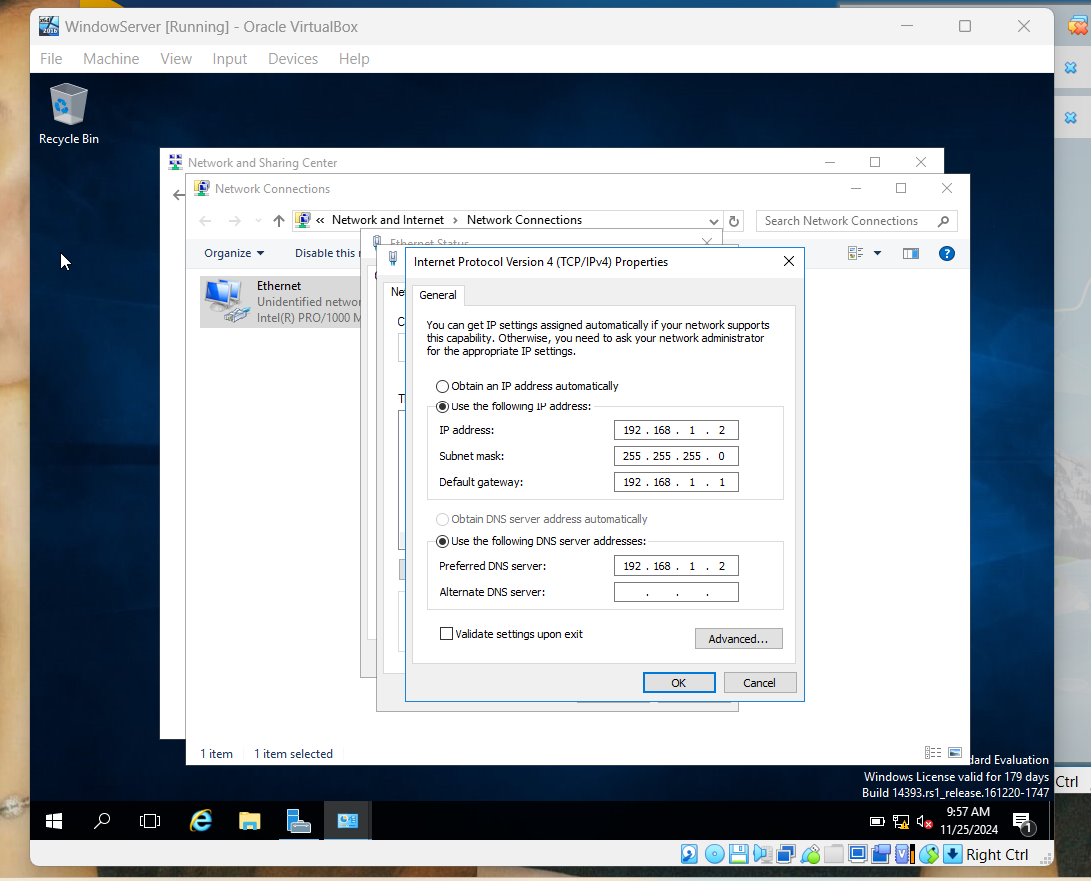
\includegraphics[width=0.5\linewidth]{RemoteAccessVPNimg/setIP_Server.png}
        \caption{Cấu hình IP cho máy WindowServer}
    \end{figure}
 \end{itemize}


  \begin{itemize}
   \item Tắt tường lửa của máy WindowServer để có thể kiểm tra đường truyền của các máy với nhau.:
   
        \begin{figure}[htbp]
        \centering
        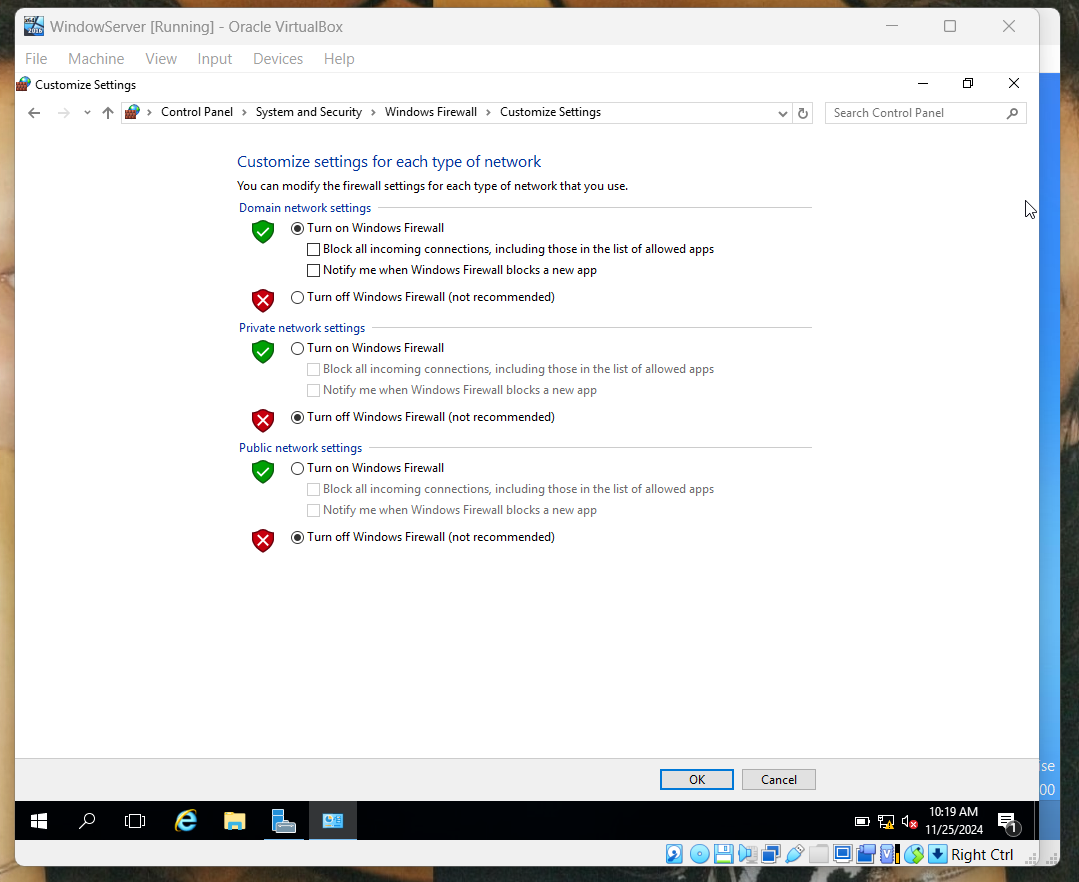
\includegraphics[width=0.6\linewidth]{RemoteAccessVPNimg/Firewall_SV.png}
        \caption{Tắt firewall WindowServer}
        \end{figure}
        
  \end{itemize}

\newpage
 \textbf{\textit{Thực hiện cấu hình Routing and Remote Access tại máy WindowServer}}

 \begin{itemize}
      \item Đầu tiên ta sẽ bắt đầu cài đặt và thiết lập Routing and Remote Access. Mở tab Server Manager > Add Roles and Features.
      \begin{figure}[htbp]
        \centering
        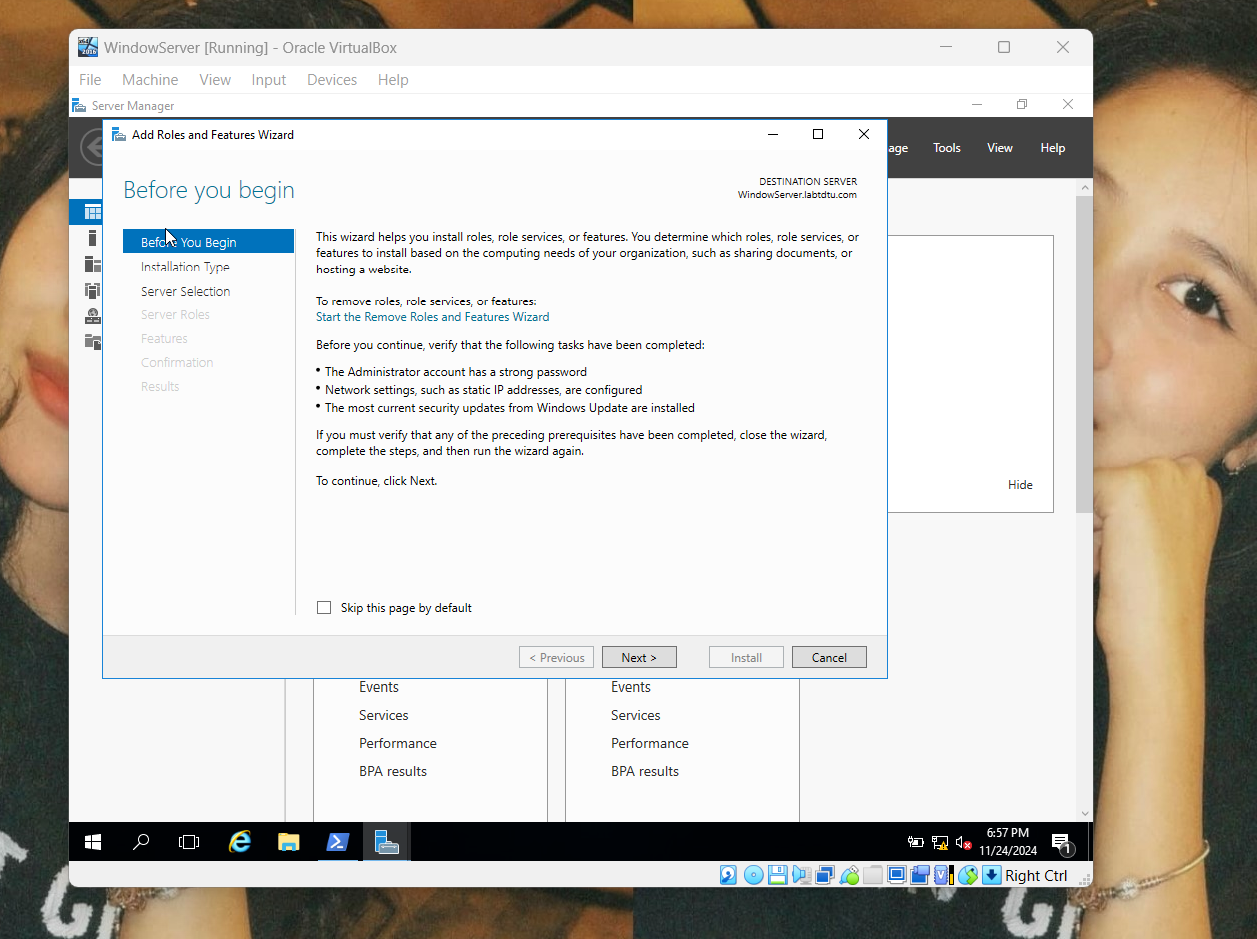
\includegraphics[width=0.6\linewidth]{RemoteAccessVPNimg/1.png}
        \caption{Cấu hình Routing and Remote Acces}
    \end{figure}
    \newpage
\item Để thêm quyền truy cập từ xa ta chọn "Remote Access" trong tab "Server Roles"

        \begin{figure}[htbp]
        \centering
        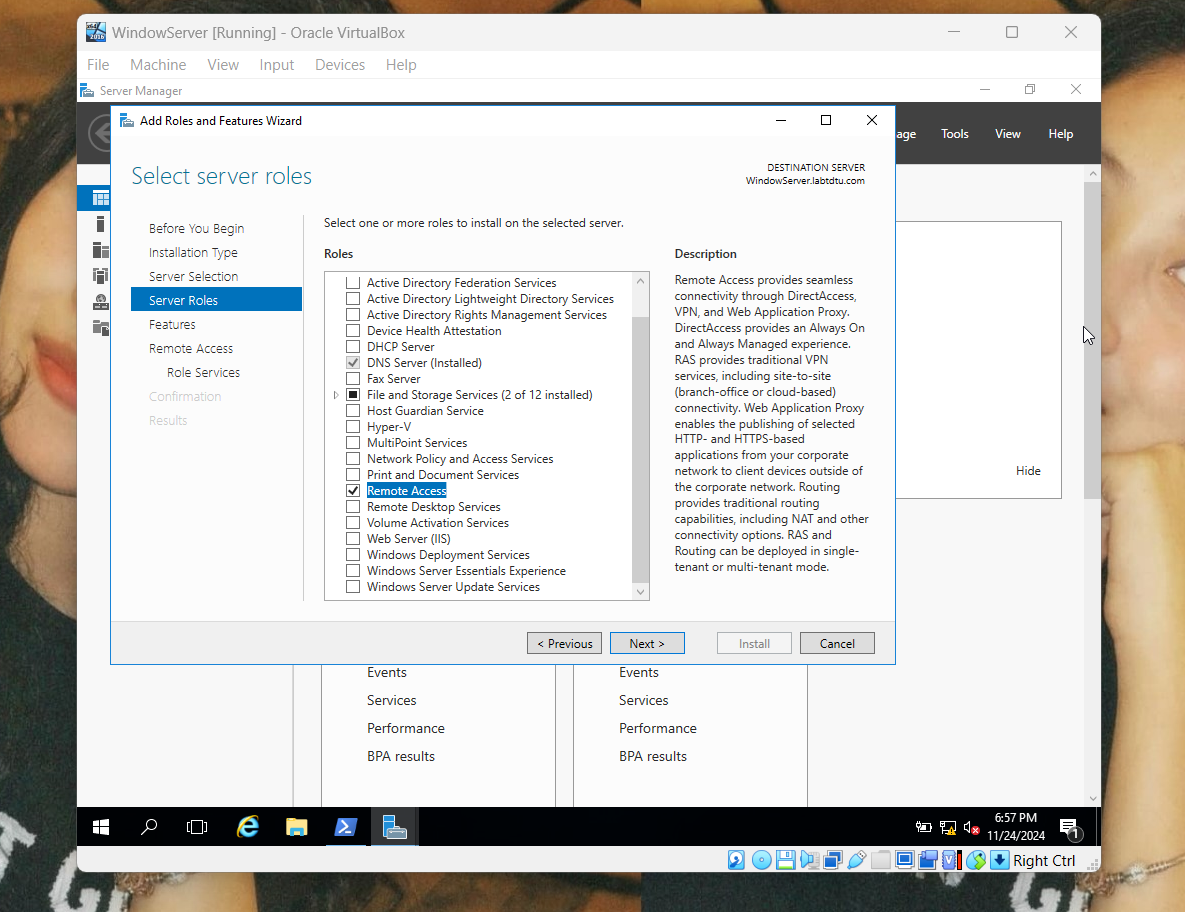
\includegraphics[width=0.6\linewidth]{RemoteAccessVPNimg/2.png}
        \caption{Thêm quyền truy cập từ xa}
        \end{figure}
\item Tại tab "Role Services" nhấn chọn "DirecAccess and VPN (RAS)" và "VPN" bởi vì ta cần các vai trò của VPN cũng như có thể cấu hình một NAT nội bộ chỉ định địa chỉ IP nội bộ. Sau đó, kiểm tra và tiến hành cài đặt.
         \begin{figure}[htbp]
            \subfloat[Cấu hình vai trò dịch vụ]
            {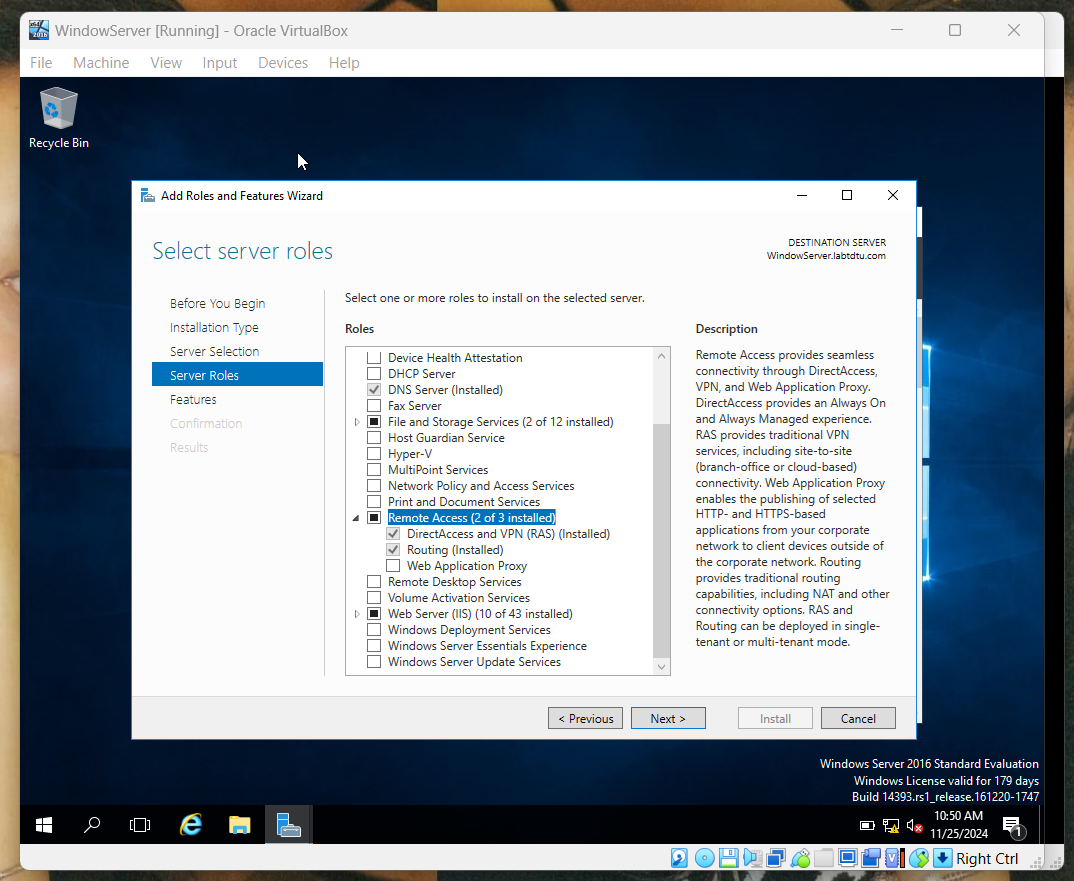
\includegraphics[width=7cm]{RemoteAccessVPNimg/3.png}}\hfill
            \subfloat[Kiểm tra]
            {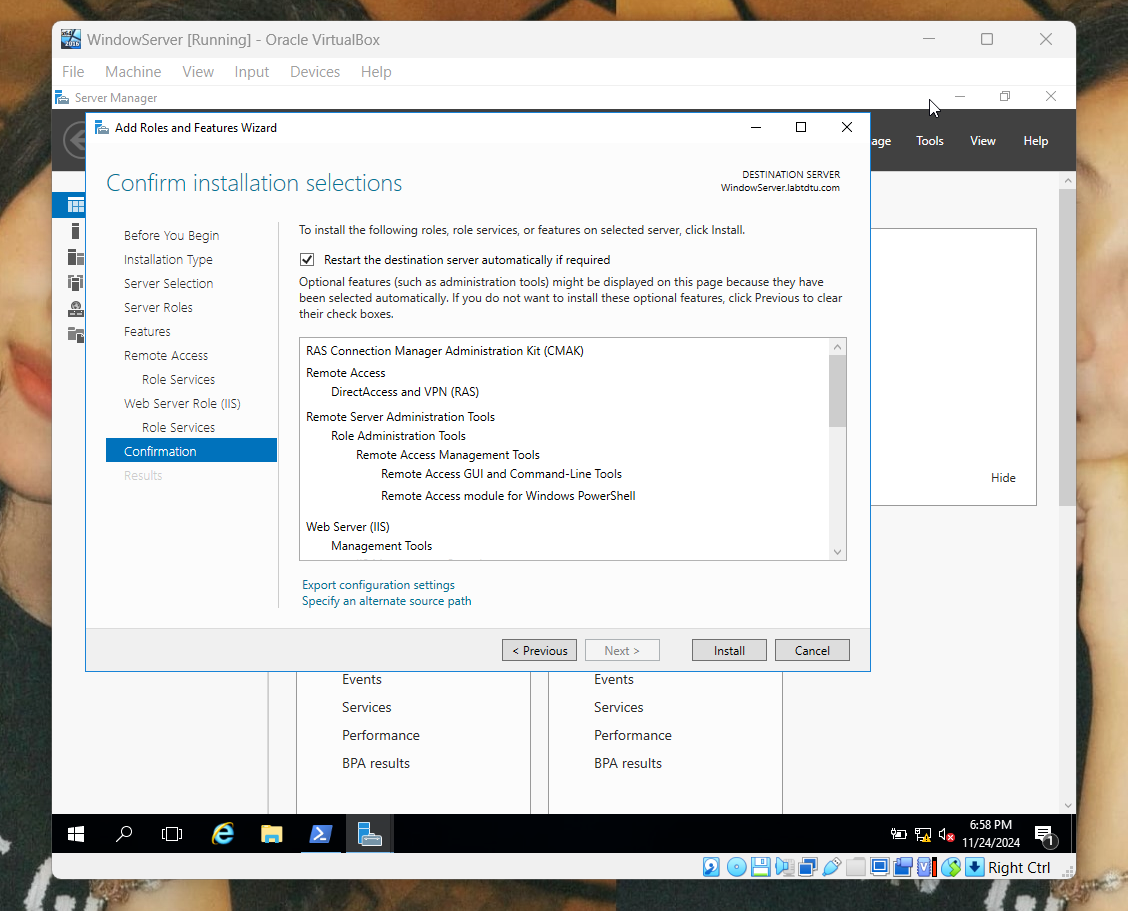
\includegraphics[width=7cm]{RemoteAccessVPNimg/4.png}}\hfill
            \caption{Cài đặt dịch vụ}
        \end{figure}
        
\newpage
\item Sau khi cài đặt thì ta có thể bắt đầu thiết lập "Routing và Remote access". Tại cửa sổ Server Manage > Tools > Routing and Remote Access. Nhấp chuột phải vào tên máy chủ > Configure and Enabling Routing and Remote Access. Lúc này cửa sổ Configure Remote Access sẽ hiển thị. 
\item Tại cửa sổ Configure Remote Access > Deploy VPN only > Next.

        \begin{figure}[htbp]
        \centering
        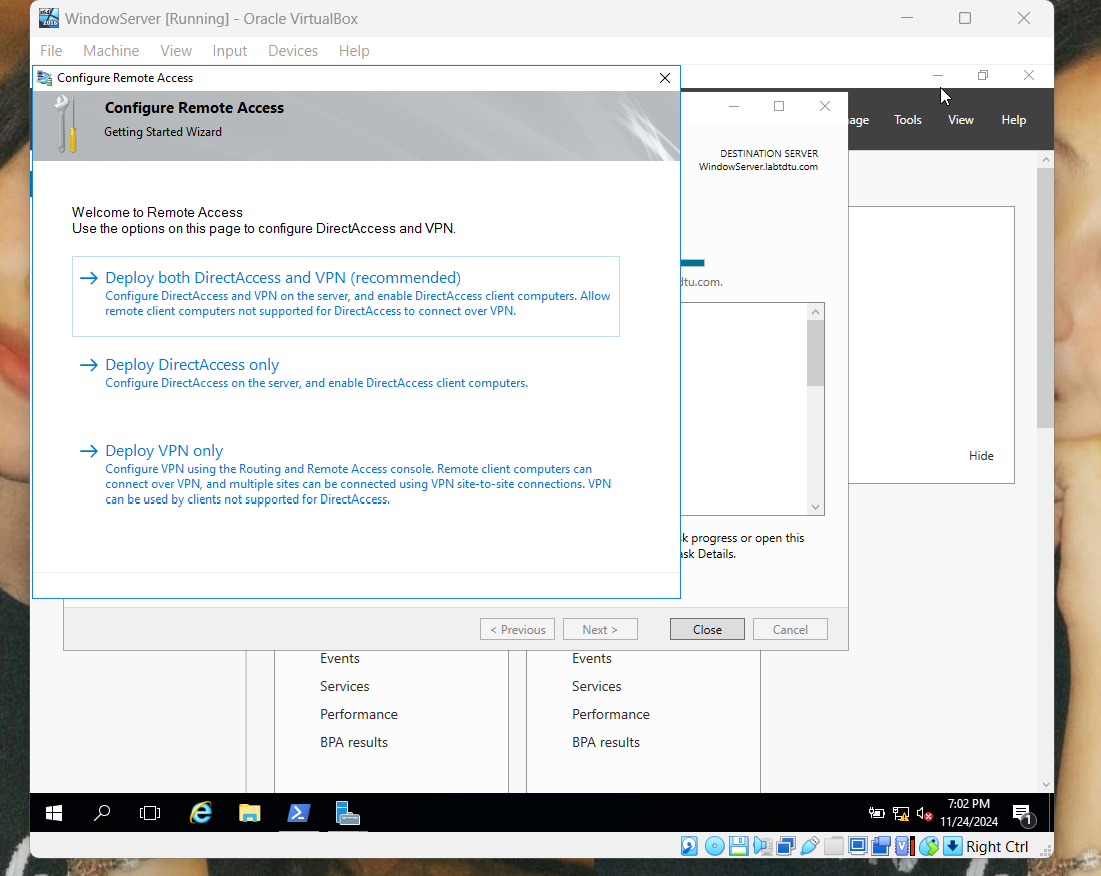
\includegraphics[width=0.5\linewidth]{RemoteAccessVPNimg/6.png}
        \caption{Configure Remote Access}
        \end{figure}
        
\item Tại cửa sổ tiếp theo, nhấn chuột vào Custom Configuration > Next.

        \begin{figure}[htbp]
        \centering
        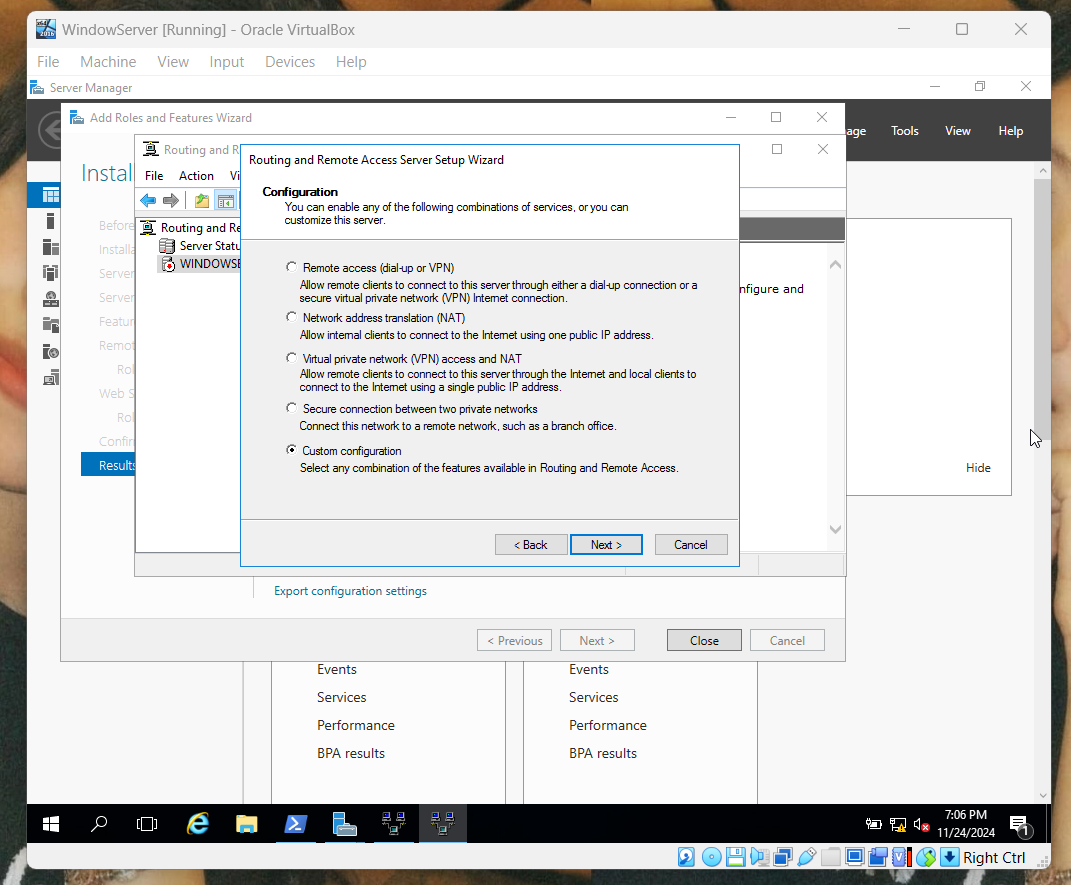
\includegraphics[width=0.5\linewidth]{RemoteAccessVPNimg/8.png}
        \caption{Custom Configuration}
        \end{figure}

\item Nhấn chuột chọn 3 dịch vụ VPN Access, Deman-dial connections, LAN Routing.
\newpage
        \begin{figure}[htbp]
        \centering
        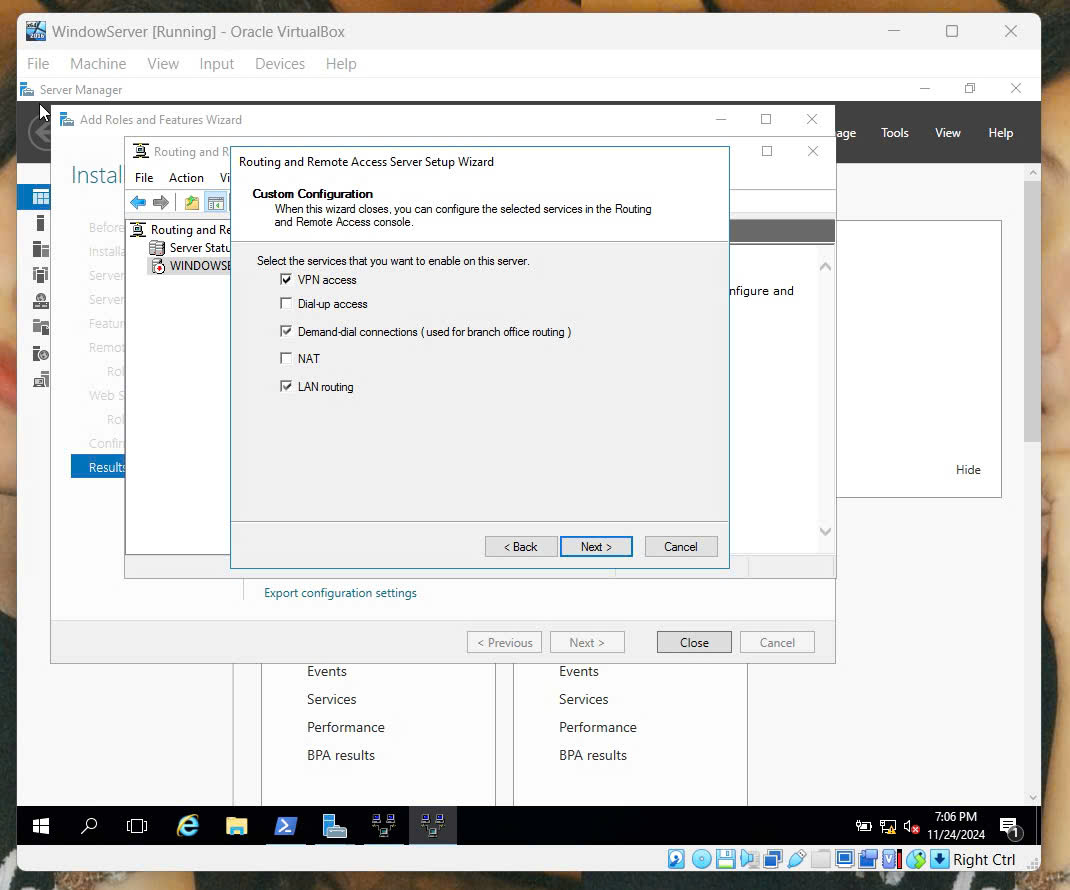
\includegraphics[width=0.5\linewidth]{RemoteAccessVPNimg/click.jpg}
        \caption{Chọn dịch vụ}
        \end{figure}

\item Sau khi chọn dịch vụ thì ta có thể bắt đầu dịch vụ và hoàn tất thiết lập

        \begin{figure}[htbp]
            \subfloat[Bắt đầu dịch vụ]
            {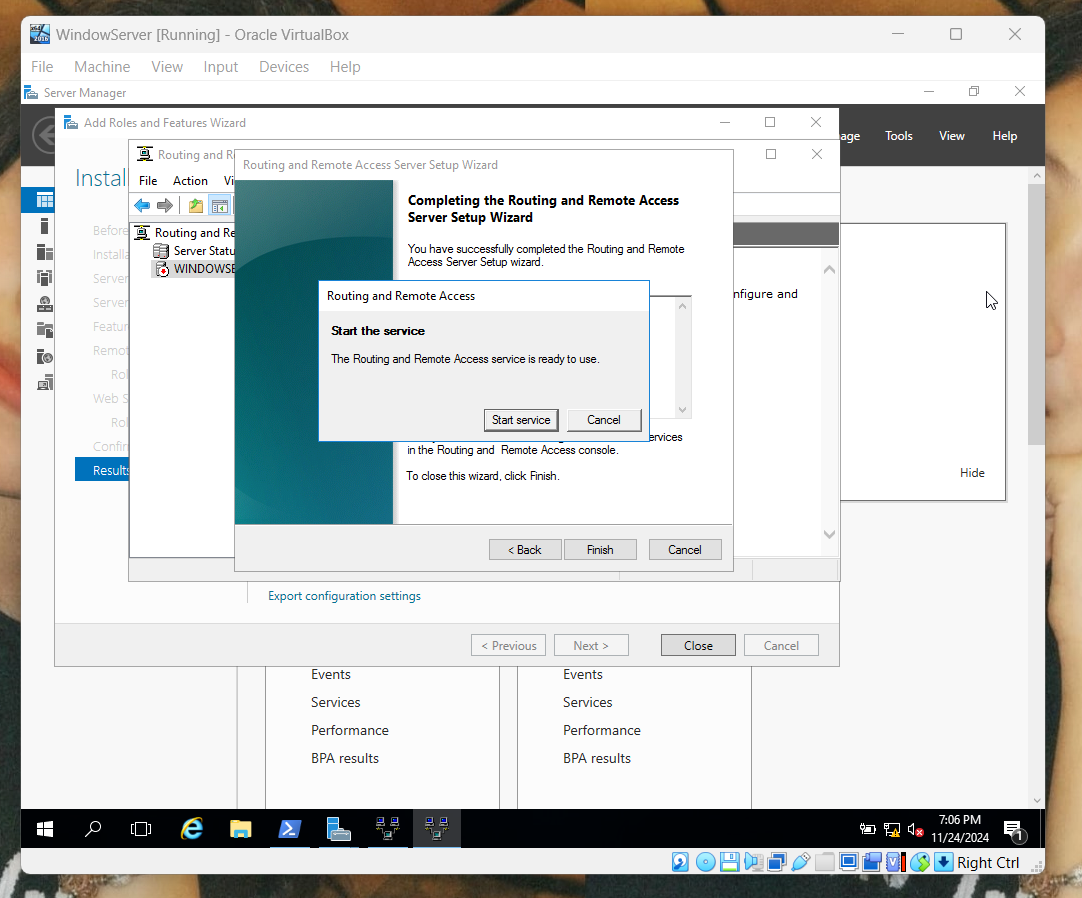
\includegraphics[width=7cm]{RemoteAccessVPNimg/9.png}}\hfill
            \subfloat[Đợi để hoàn tất thiết lập]
            {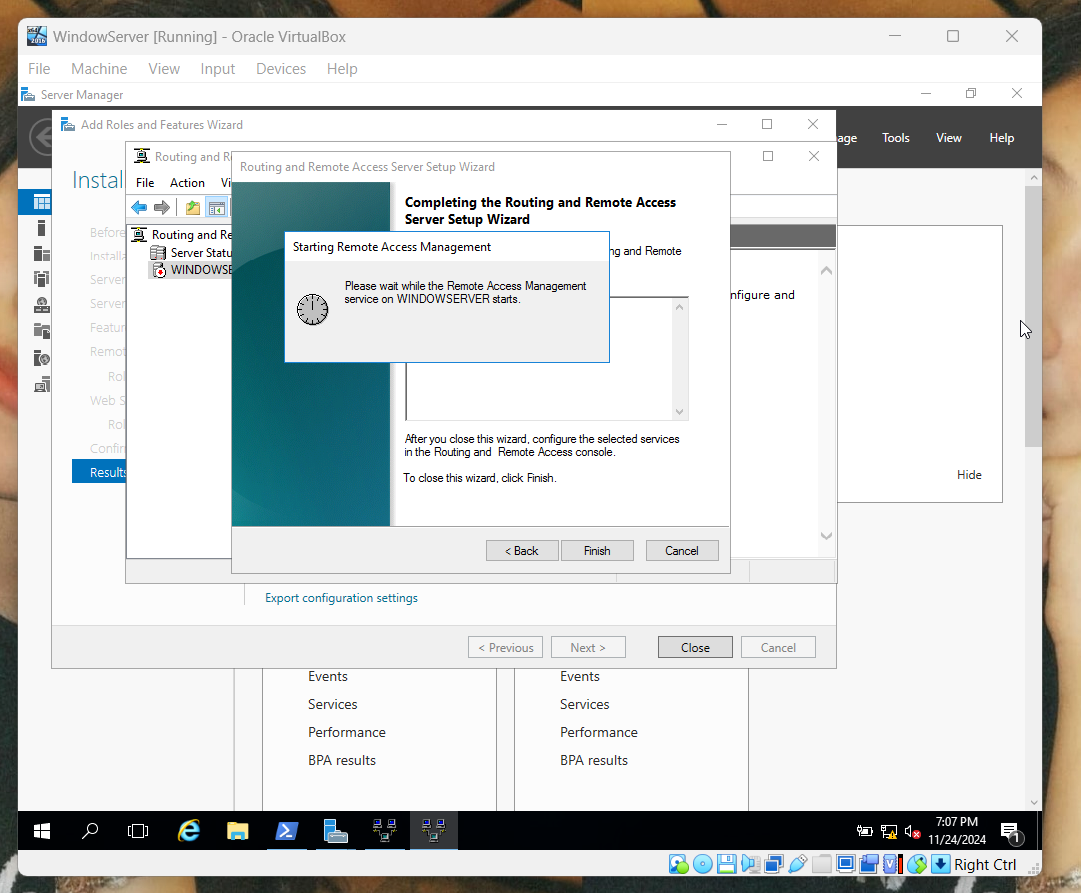
\includegraphics[width=7cm]{RemoteAccessVPNimg/10.png}}\hfill
            \caption{Hoàn tất thiết lập Routing And Remote Access}
        \end{figure}

\end{itemize}

 \textbf{\textit{Tiến hành cài đặt dải địa chỉ Ipv4 tại máy WindowServer}}

  \begin{itemize}
      \item Mở cửa sổ Routing and Remote Access: Server Manager > Tools > Routing and Remote Access. Tại đây ta nhấp chuột phải vào tên máy chủ và đi đến Properties.
    \item Nhấn chuột vào tab Ipv4. Tại khung Ipv4 address assignment: Static address pool > Add. Sau đó nhập vào dài địa chỉ Ipv4.
   \newpage   
      \begin{figure}[htbp]
            \subfloat[Thao thác thiết lập dải địa chỉ Ipv4]
            {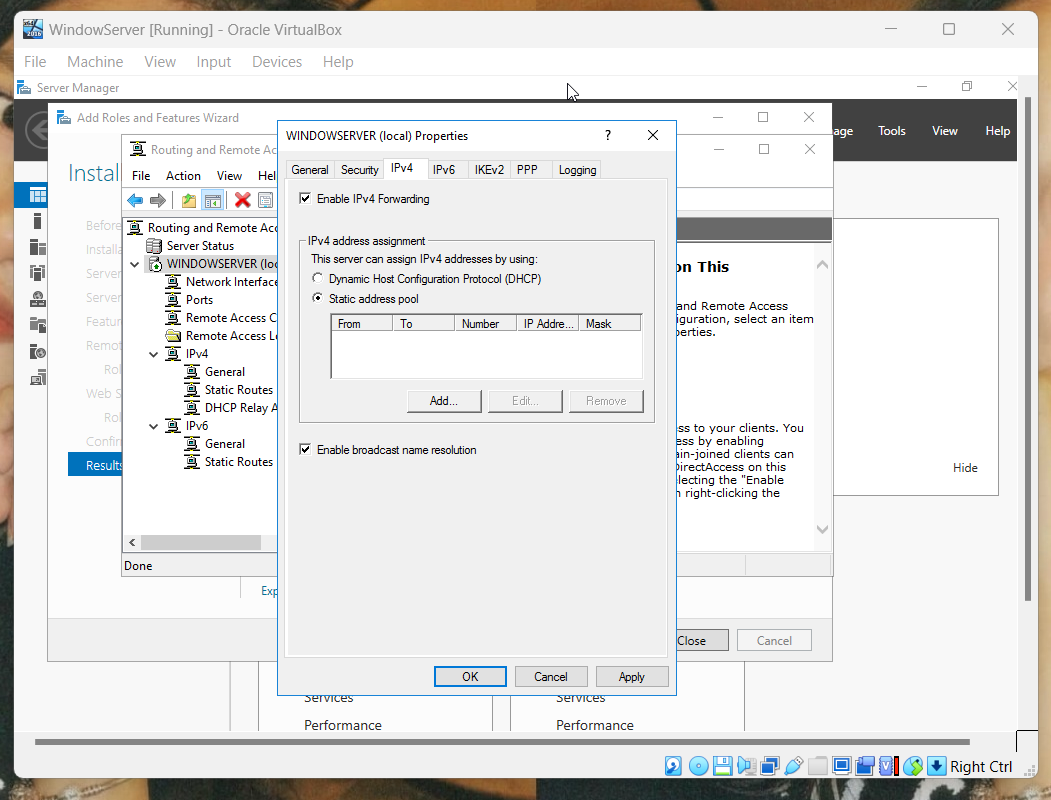
\includegraphics[width=7cm]{RemoteAccessVPNimg/setDaiIP.png}}\hfill
            \subfloat[Nhập dải địa chỉ Ipv4]
            {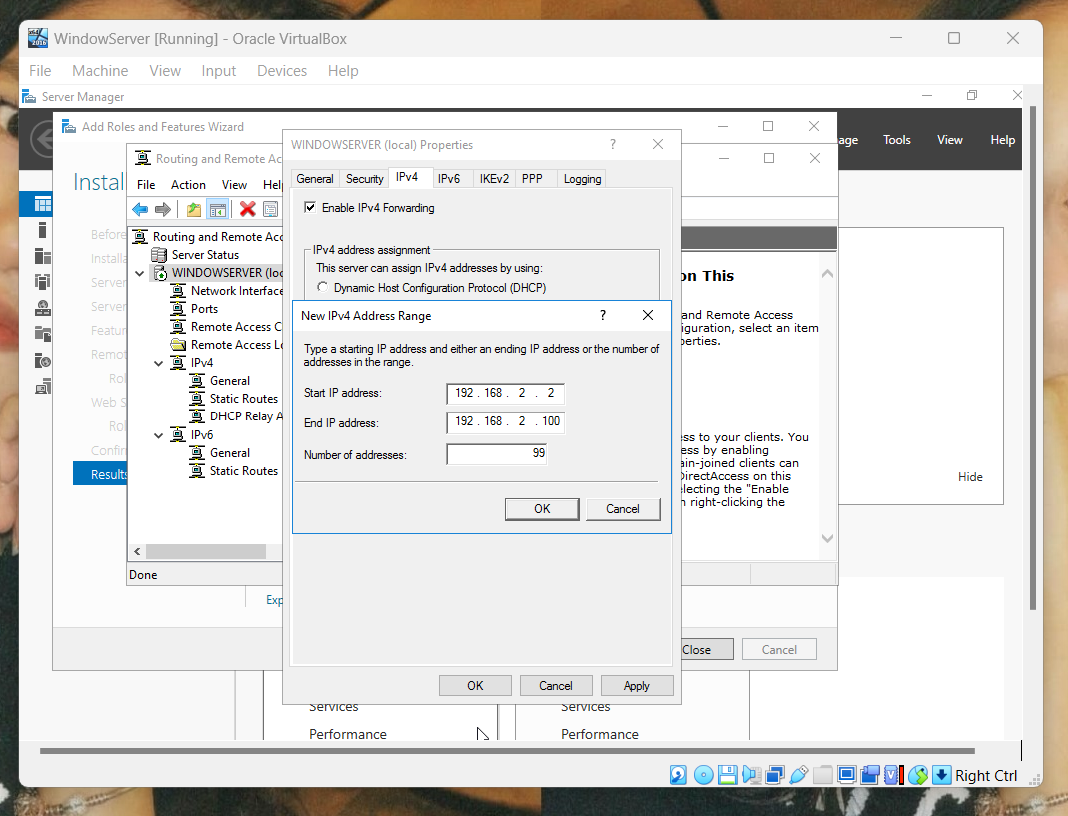
\includegraphics[width=7cm]{RemoteAccessVPNimg/setDaiIP_1.png}}\hfill
            \caption{Cài đặt dải địa chỉ Ipv4}
        \end{figure}

 \end{itemize}

 \textbf{\textit{Tạo người dùng tại máy WindowServer}}
 
  \begin{itemize}
      \item Mở cửa sổ Active Directory Users And Computers: Server Manager > Tools > Active Directory Users And Computers. Chọn labtdtu.com và nhấn chuột phải > New > Organizational Unit.

    \begin{figure}[htbp]
        \centering
        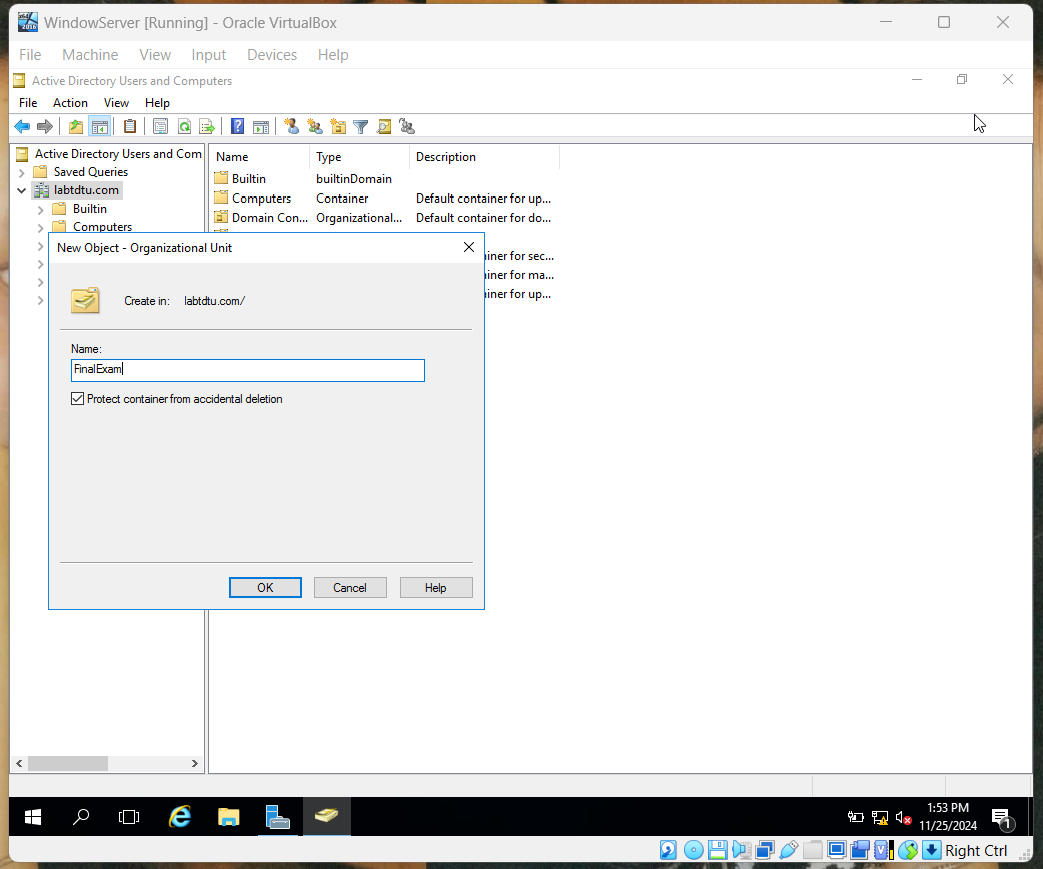
\includegraphics[width=0.5\linewidth]{RemoteAccessVPNimg/createOU.png}
        \caption{Tạo OU mới}
    \end{figure}
      
    \item Tại OU FinalExam mới được tạo, nhấn chuột phải > New > User. Sau đó nhập các thông tin vào các ô trống, nhấn chọn Next > Finish để tạo User mới.
\newpage
    \begin{figure}[htbp]
            \subfloat[Nhập thông tin để tạo User mới]
            {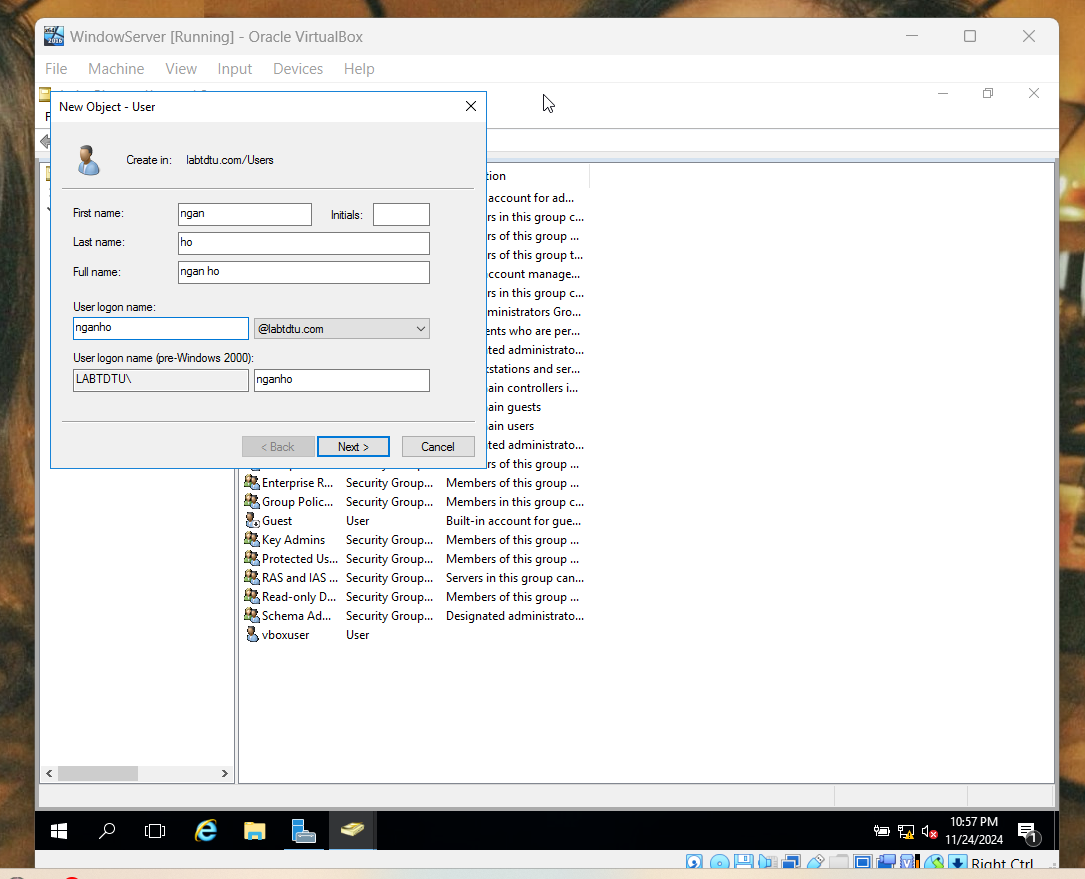
\includegraphics[width=7cm]{RemoteAccessVPNimg/CreateUser_SV1.png}}\hfill
            \subfloat[Nhấn chọn Finish]
            {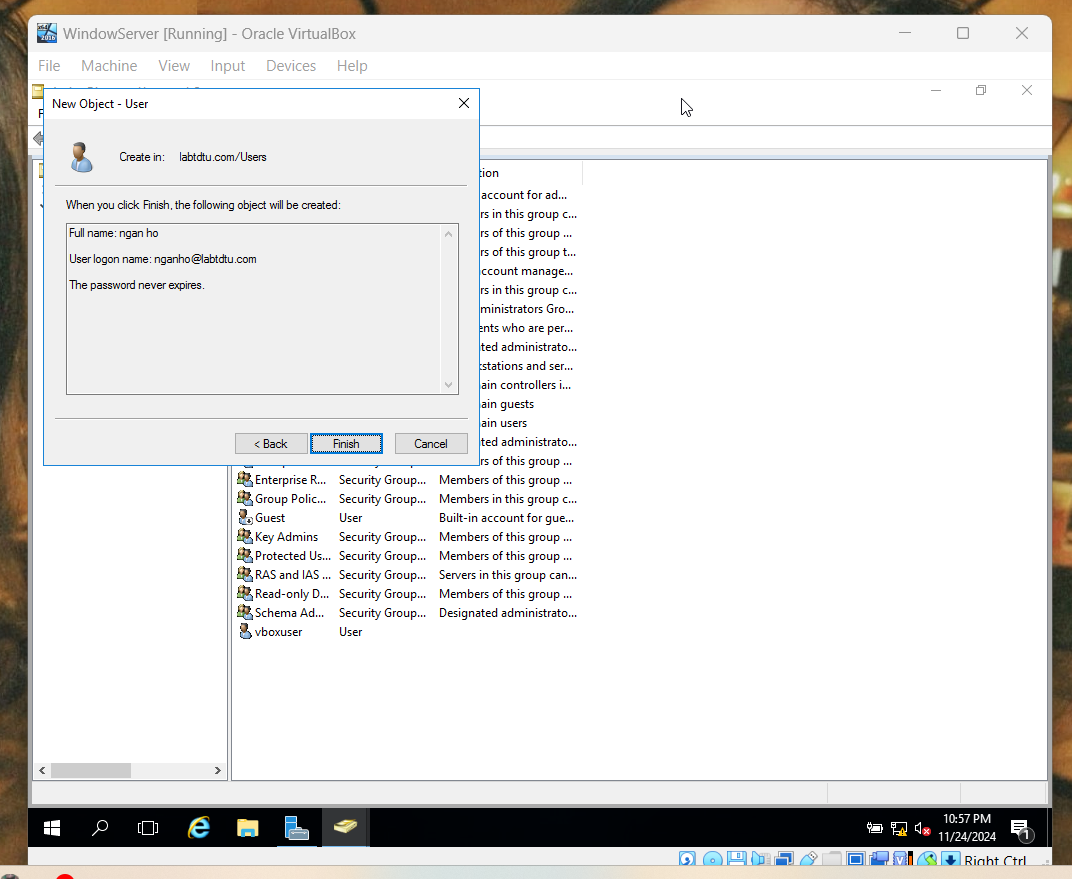
\includegraphics[width=7cm]{RemoteAccessVPNimg/CreateUser_SV2.png}}\hfill
            \caption{Tạo User}
        \end{figure}

 \end{itemize}

 \textbf{\textit{Tạo thư mục tại máy WindowServer và cho phép user truy cập từ xa vào lấy tài liệu}}

   \begin{itemize}
      \item Tại ổ đĩa C của máy WindowServer, tạo 1 thư mục "Text". Trong thư nục "Text" tạo 1 tệp tin "XinChao".

    \begin{figure}[htbp]
        \centering
        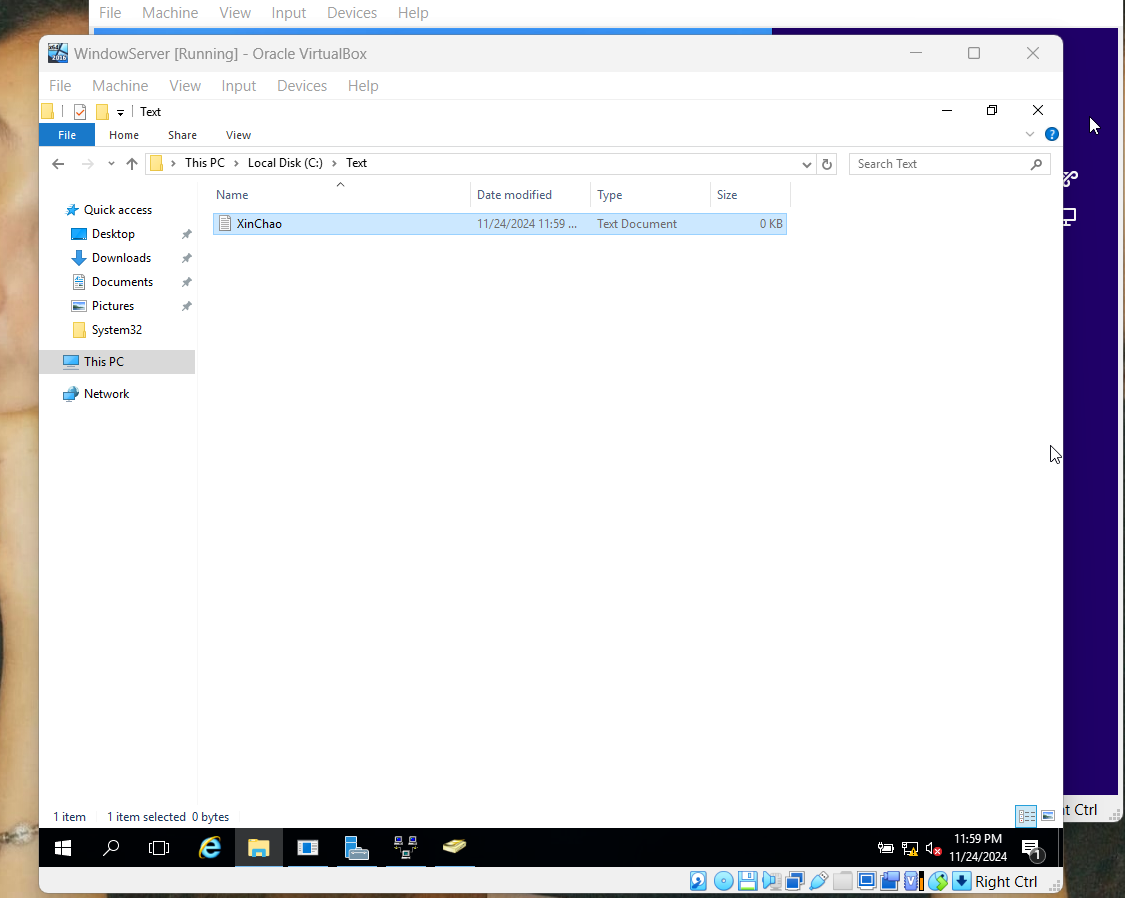
\includegraphics[width=0.6\linewidth]{RemoteAccessVPNimg/CreateFile_SV.png}
        \caption{Tạo tệp tin}
    \end{figure}
\newpage
    \item Sau khi tạo xong tệp tin trong thư mục Text. Ta trở về thư mục, nhấn chuột phải vào thư mục Text > Properties > Security > Edit > Add > Điền "Everyone" vào ô Enter the object names to select > Ok.

    \begin{figure}[htbp]
        \centering
        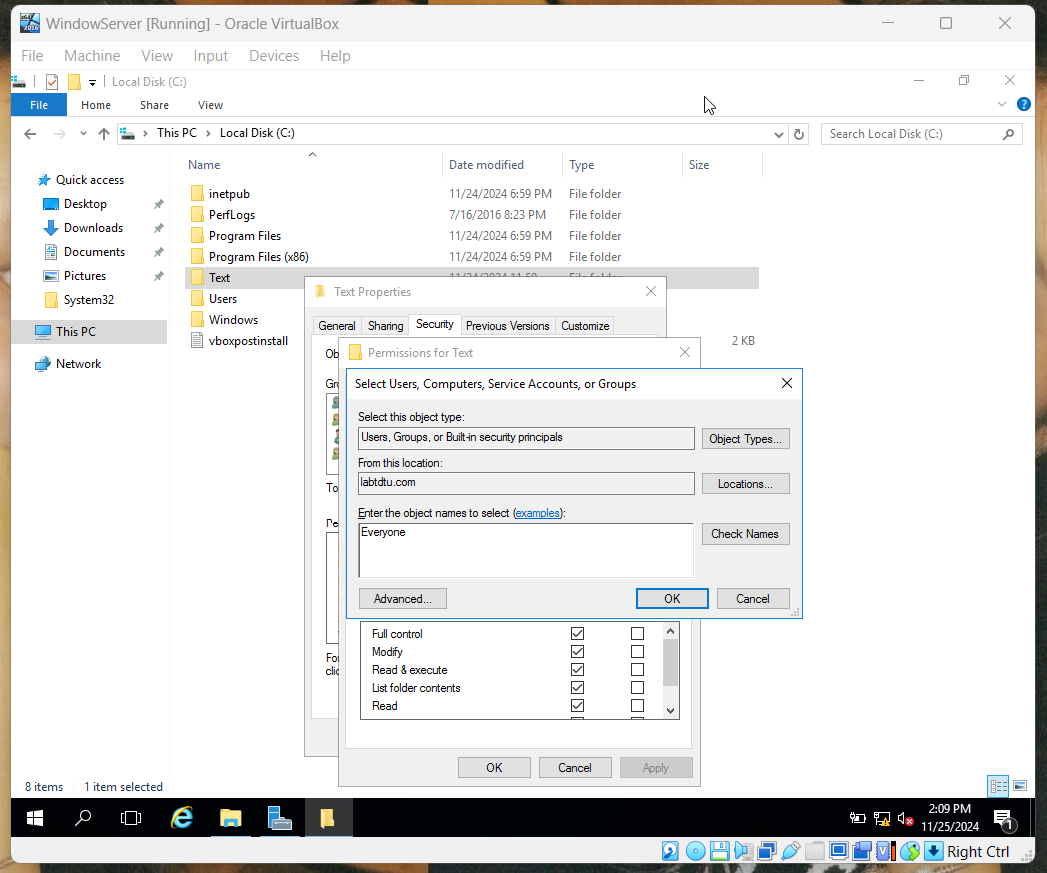
\includegraphics[width=0.6\linewidth]{RemoteAccessVPNimg/ShareFile_SV (3).png}
        \caption{Chia sẻ tệp tin}
    \end{figure}

    \item Tiếp theo, trong cửa sổ Properties > Sharing > Share > Everyone > Share.

    \begin{figure}[htbp]
        \centering
        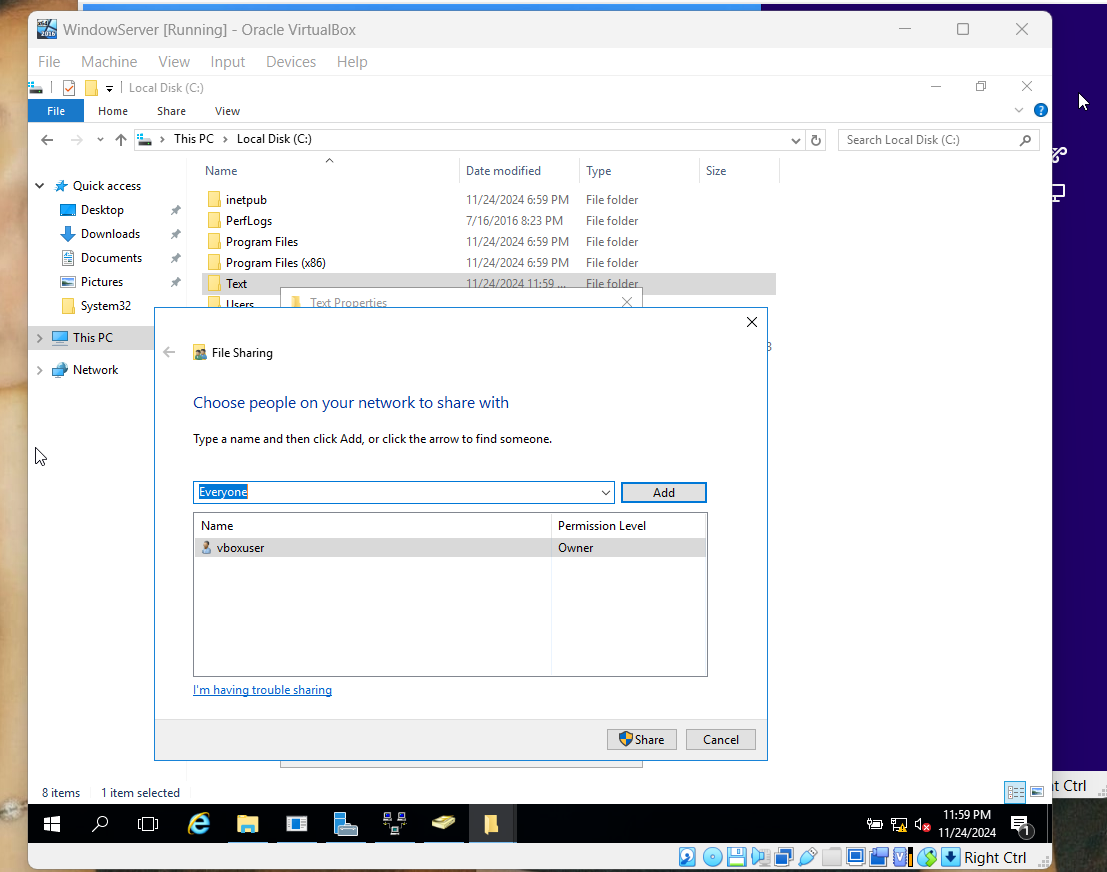
\includegraphics[width=0.6\linewidth]{RemoteAccessVPNimg/ShareFile_SV (2).png}
        \caption{Chia sẻ tệp tin}
    \end{figure}
 \end{itemize}

\newpage
\textbf{\textit{Thực hiện cấu hình IP tại máy Client1}}
\begin{itemize}
      \item Cài đặt địa chỉ IP cho máy Client1

    \begin{figure}[htbp]
        \centering
        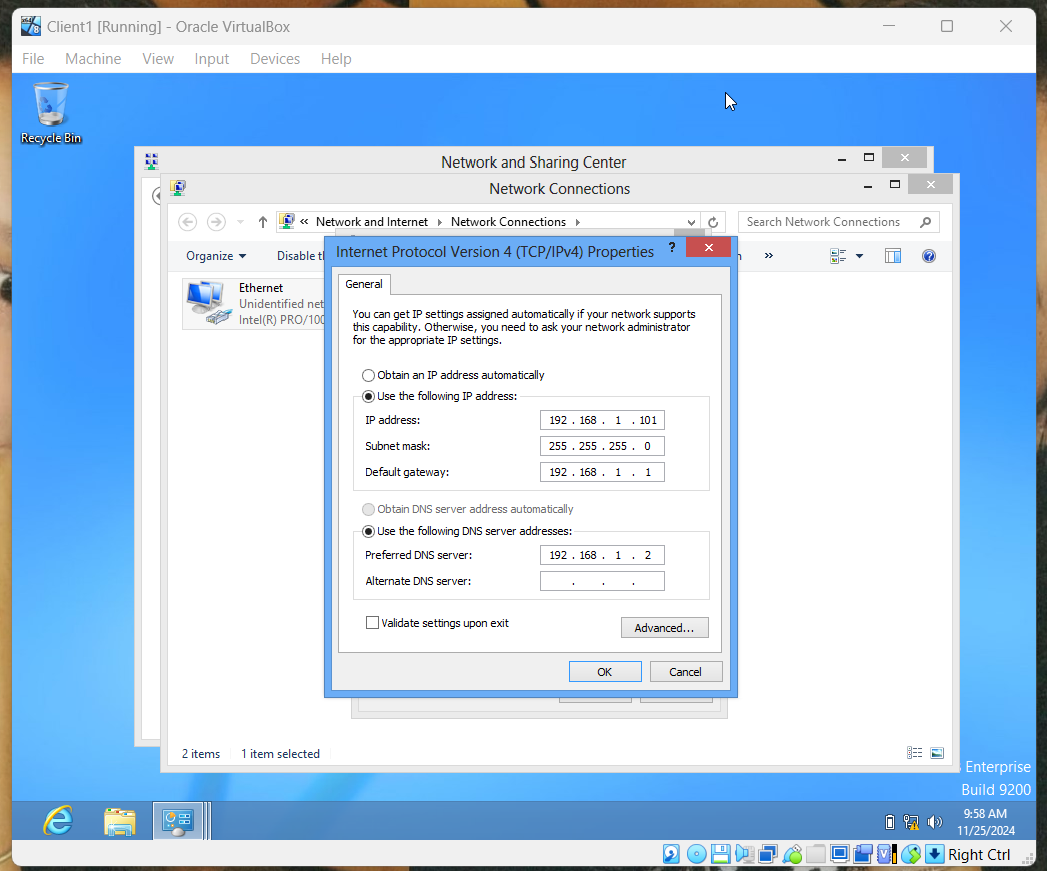
\includegraphics[width=0.5\linewidth]{RemoteAccessVPNimg/setIP_CLient.png}
        \caption{Cấu hình IP cho máy Client1}
    \end{figure}
      
    \item Tắt tường lửa của máy Client1 để có thể kiểm tra đường truyền của các máy với nhau 

    \begin{figure}[htbp]
        \centering
        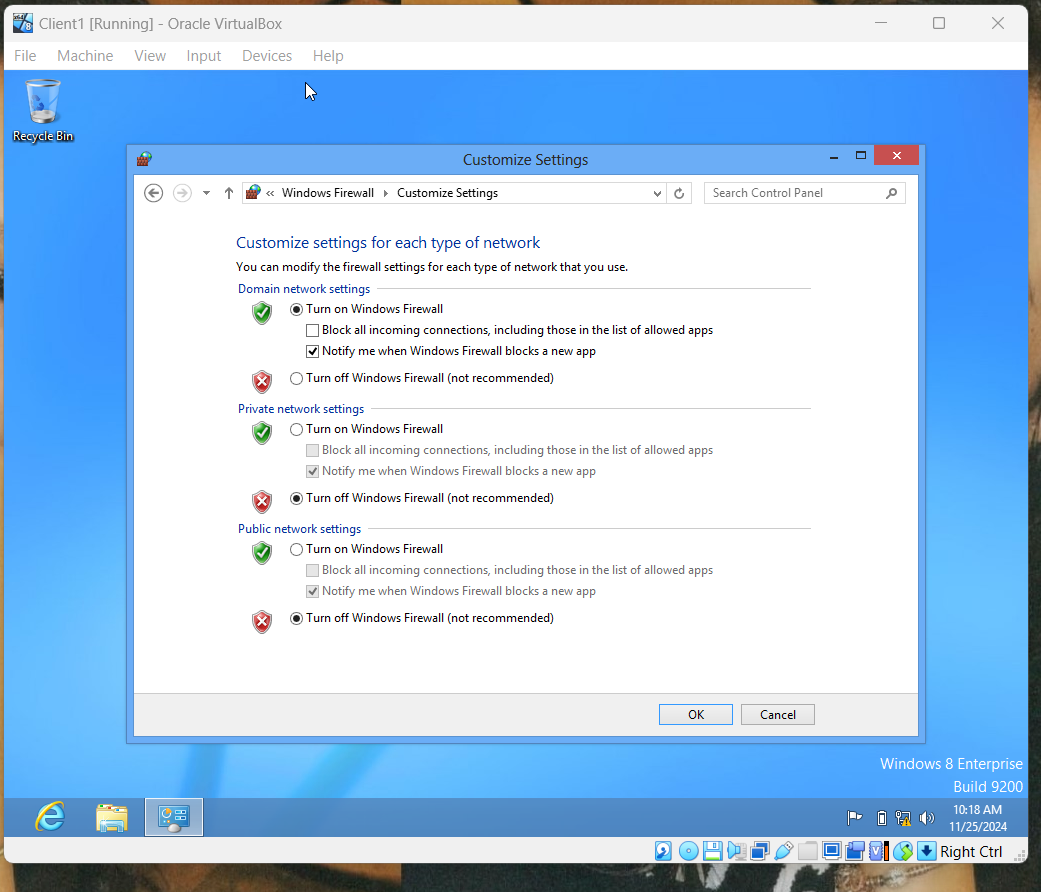
\includegraphics[width=0.5\linewidth]{RemoteAccessVPNimg/Firewall_Client.png}
        \caption{Tắt tường lửa tại máy Client1}
    \end{figure}
 \end{itemize}


\subsubsection*{4.1.1.3 Thực nghiệm}
 \addcontentsline{toc}{subsubsection}{4.1.1.3 Thực nghiệm}
 
\textbf{\textit{Tiến hành cho máy CLient1 join vào VPN}}
\begin{itemize}
      \item Mở Control Pannel > Network And Internet > Network And Sharing Centre > Set up a Connection or Network > Connect to a WorkPlace > Next. 
      \newpage
    \begin{figure}[htbp]
            \subfloat[Thao tác 1]
            {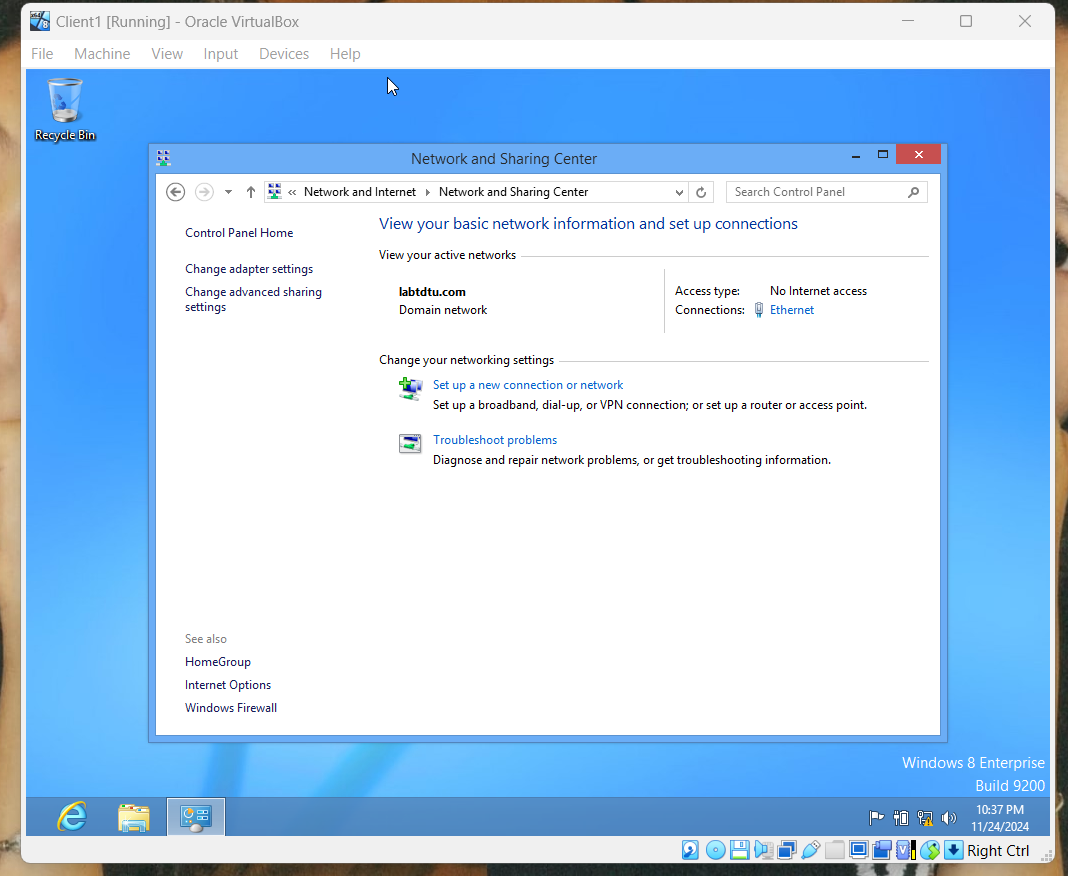
\includegraphics[width=7cm]{RemoteAccessVPNimg/ClientJoinVPN_3.png}}\hfill
            \subfloat[Thao tác 2]
            {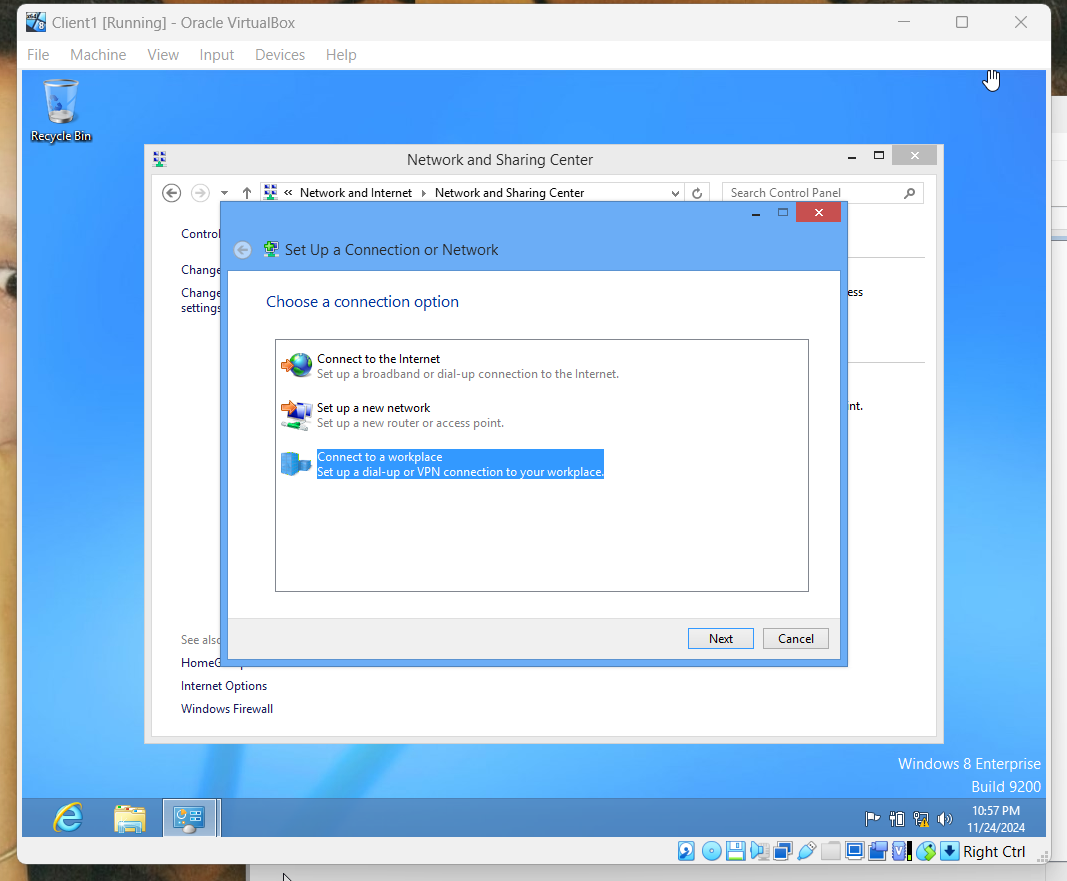
\includegraphics[width=7cm]{RemoteAccessVPNimg/ClientJoinVPN_1.png}}\hfill
            \caption{Thao tác join vào VPN}
        \end{figure}
        
    \item Tại cửa sổ Connect a workplace, nhập các thông tin vào ô trống > Create.

    \begin{figure}[htbp]
        \centering
        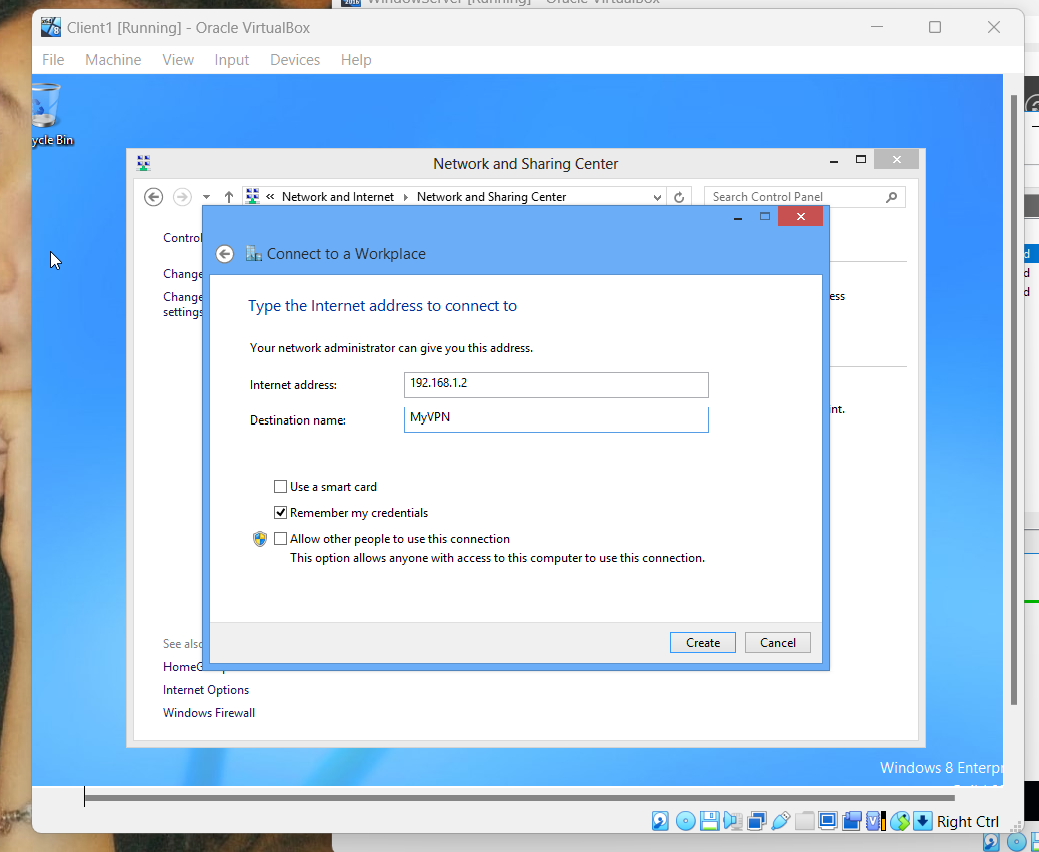
\includegraphics[width=0.7\linewidth]{RemoteAccessVPNimg/ClientJoinVPN_2.png}
        \caption{Thao tác join vào VPN}
    \end{figure}
\newpage
    \item Sau đó nhập Username và Password vào và chọn Connect.

     \begin{figure}[htbp]
            \subfloat[Chọn MyVPN để kết nối]
            {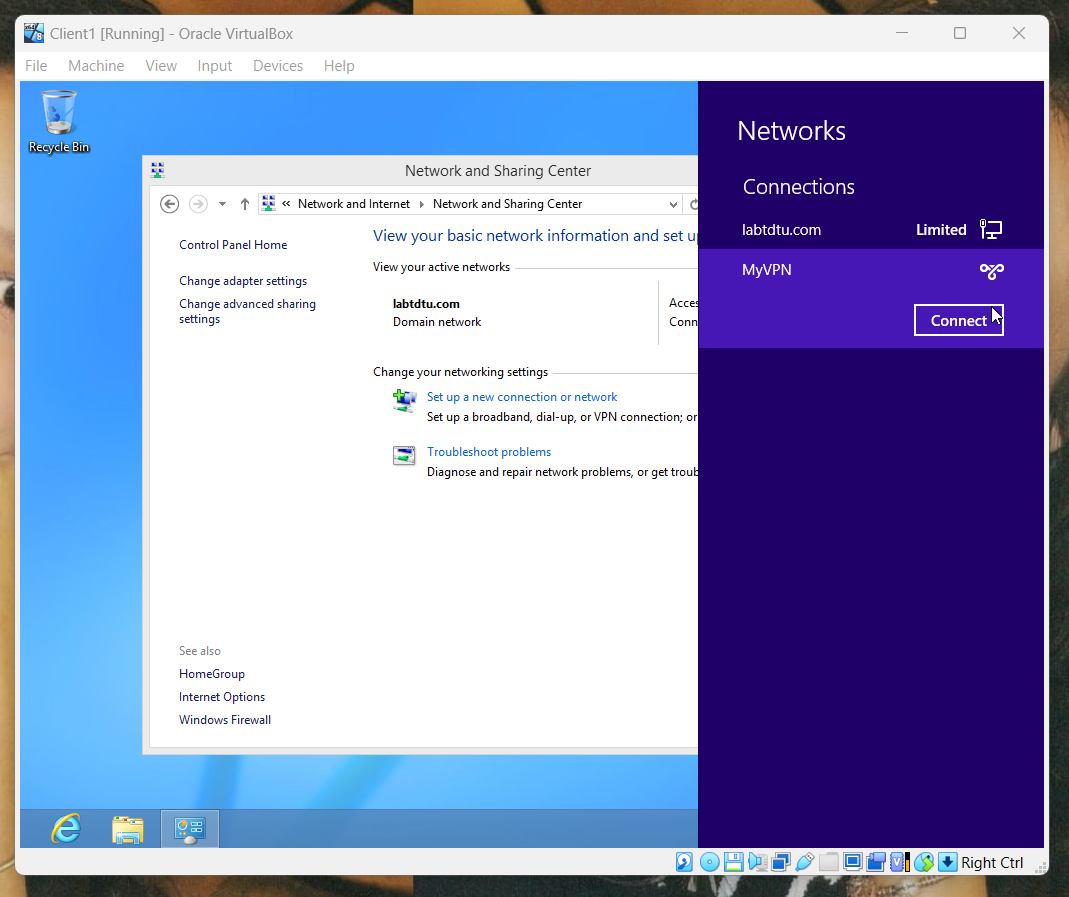
\includegraphics[width=7cm]{RemoteAccessVPNimg/ClientJoinVPN_4.png}}\hfill
            \subfloat[Kết nối thành công]
            {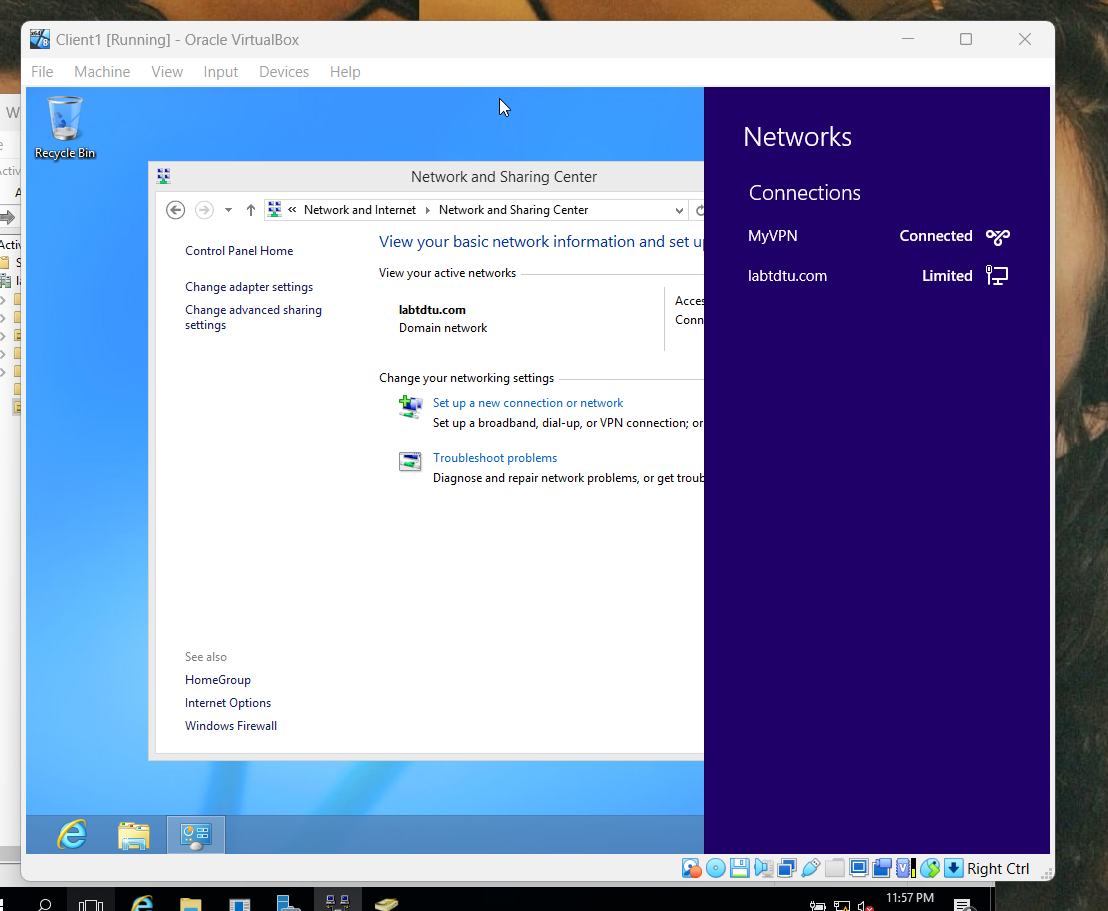
\includegraphics[width=7cm]{RemoteAccessVPNimg/ClientJoinVPN_5.png}}\hfill
            \caption{Kết nối thành công vào VPN}
        \end{figure}
 \end{itemize}

\textbf{\textit{Tiến hành cho máy Client1 truy cập vào thư mục của máy WindowServer và lấy dữ liệu}}
 
\begin{itemize}
      \item Tìm kiếm thư mục của Server: Mở hộp thoại Run > Nhập vào ô Open: \\192.168.1.2 > Ok.

    \begin{figure}[htbp]
        \centering
        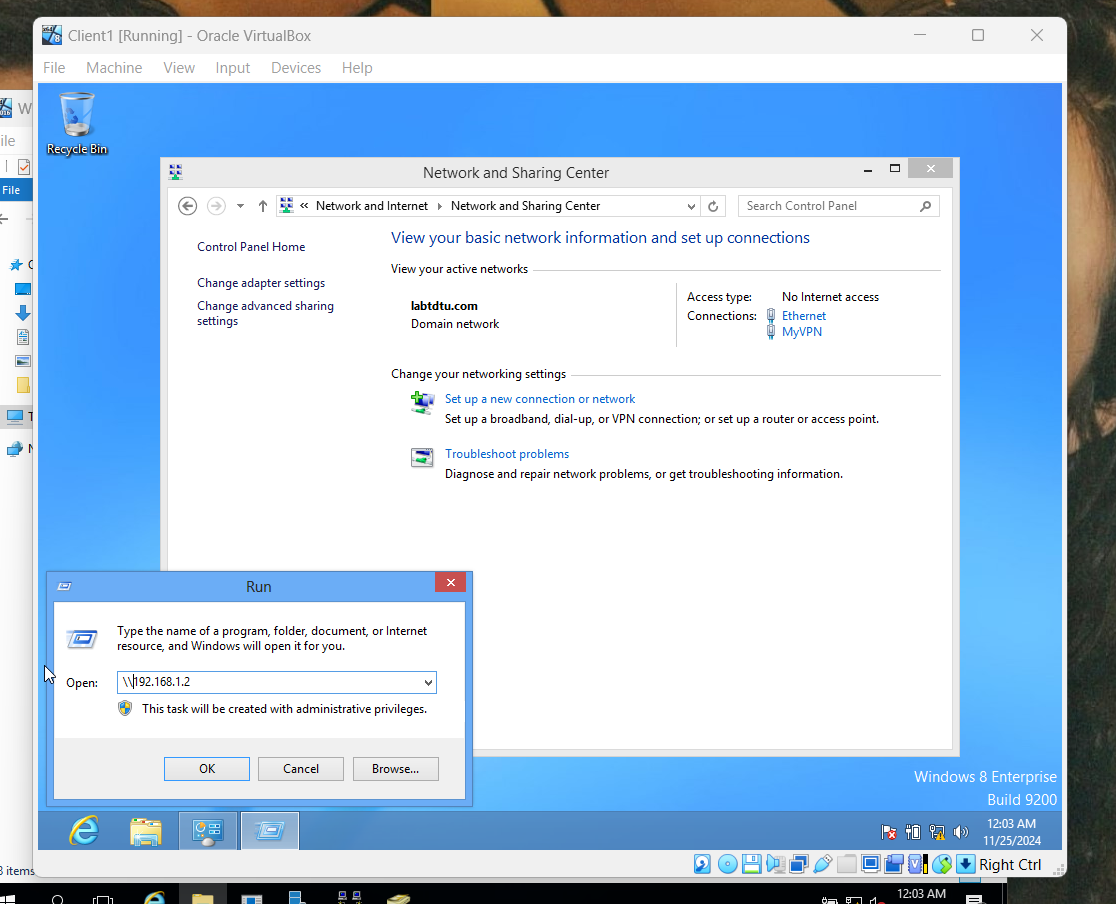
\includegraphics[width=0.6\linewidth]{RemoteAccessVPNimg/FindFile.png}
        \caption{Tìm kiếm thư mục ở máy Server}
    \end{figure}
      
    \item Tại cửa sổ mới sẽ hiển thị các thư mục được chia sẻ với máy Client1. Nhấn chuột chọn thư mục Text, trong thư mục Text sẽ hiển thị tệp tin XinChao. 

     \begin{figure}[htbp]
            \subfloat[Các thư mục được chia sẻ với Client1]
            {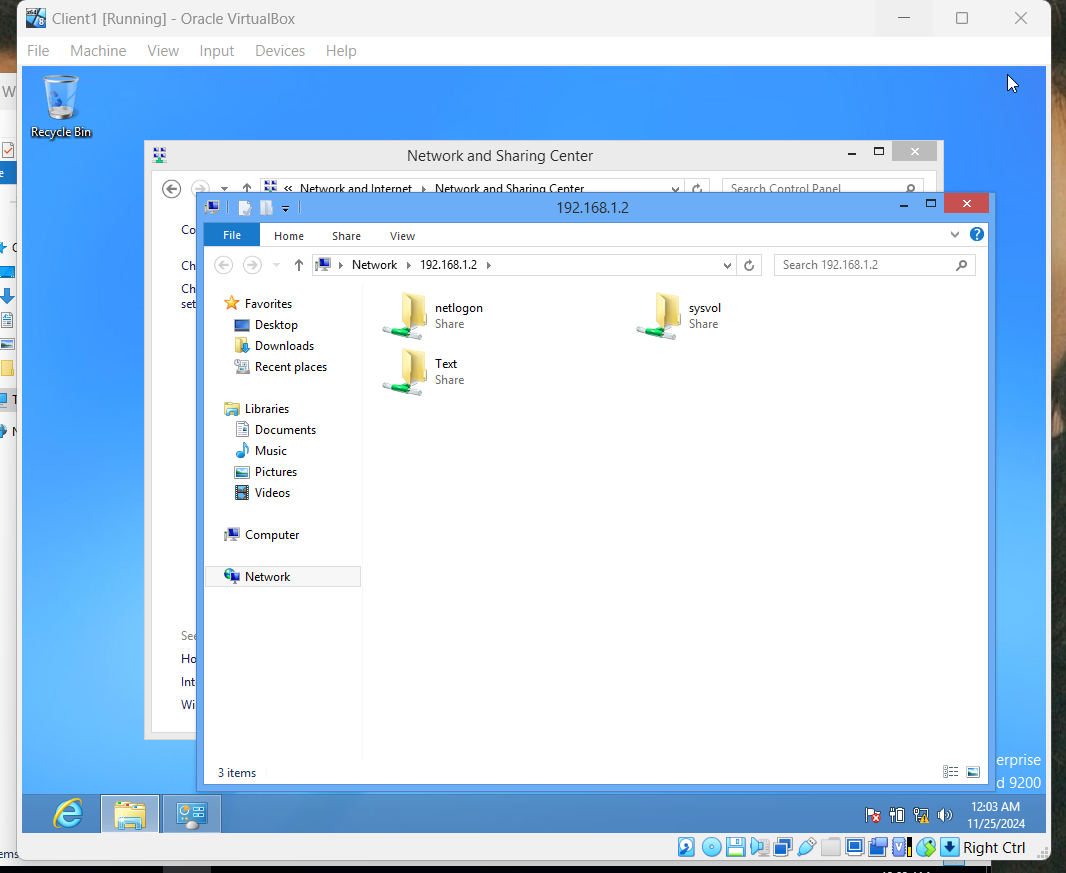
\includegraphics[width=7cm]{RemoteAccessVPNimg/FindFile (2).png}}\hfill
            \subfloat[Lấy tệp tin thành công]
            {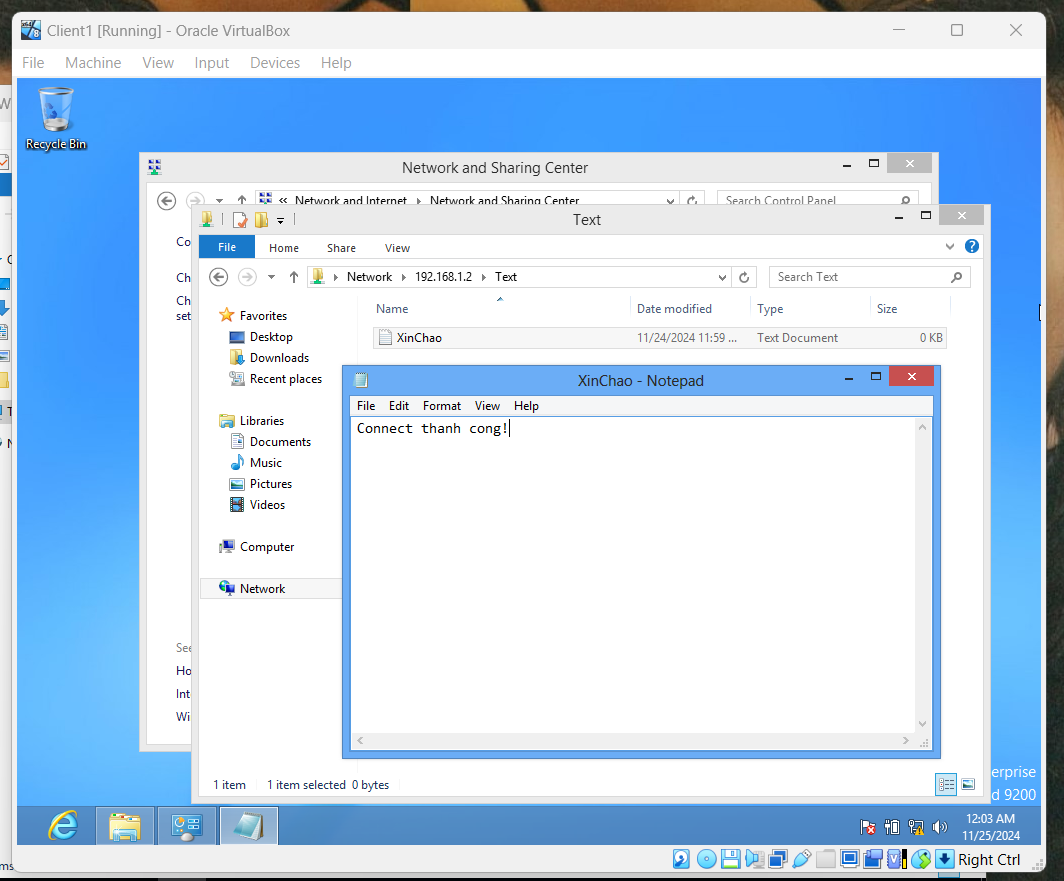
\includegraphics[width=7cm]{RemoteAccessVPNimg/Client_ConnectThanhCong.png}}\hfill
            \caption{Truy cập và lấy dữ liệu thành công}
        \end{figure}
 \end{itemize}

 \subsection*{4.1.2 Xây dựng Site-to-Site VPN}
 \addcontentsline{toc}{subsection}{4.1.2 Xây dựng Site-to-Site VPN}

  \subsubsection*{4.1.2.1 Chuẩn bị thiết bị}
 \addcontentsline{toc}{subsubsection}{4.1.2.1 Chuẩn bị thiết bị}
 \begin{itemize}
     \item Một máy chủ HN\_SVR để quản lý VPN Server ở Hà Nội.
     \item Một máy chủ TPHCM\_SVR để quản lý  VPN Server ở TP.Hồ Chí Minh.
     \item Một máy File Server dùng dể quản lý các tài liệu, data của chi nhánh Hà Nội.
     \item Một máy trạm ở TP.Hồ Chí Minh.
 \end{itemize}

\subsubsection*{4.1.2.2 Mô hình mạng}
 \addcontentsline{toc}{subsubsection}{4.1.2.2 Mô hình mạng}

Dưới đây là mô hình triển khai VPN và địa chỉ IP cho từng thiết bị. Chi nhánh tại Hà Nội có đường mạng được chia ở lớp C, còn chi nhánh TP. Hồ Chí Minh có đường mạng thuộc lớp A. Điều này sẽ làm cho mô hình được triển khai đa dạng về lớp mạng, ứng dụng thực tế.

\begin{figure}[htbp]
    \centering
    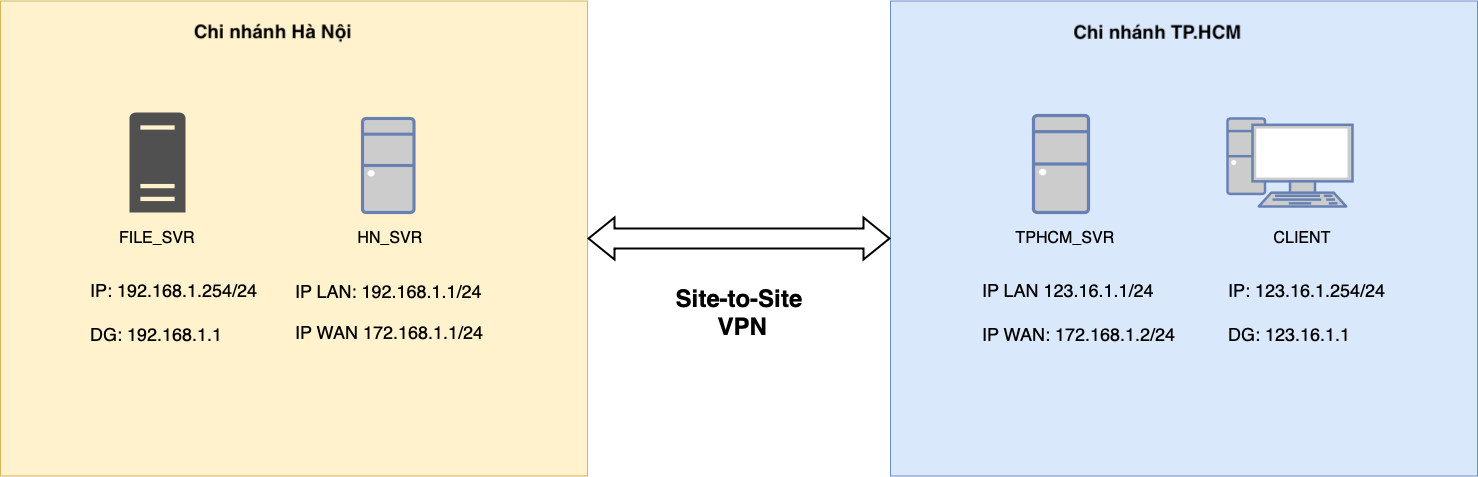
\includegraphics[width=0.9\linewidth]{img/site-to-site.png}
    \caption{Mô hình mạng triển khai VPN}
\end{figure}
\newpage
\subsubsection*{4.1.2.3 Thực hiện cấu hình}
 \addcontentsline{toc}{subsubsection}{4.1.2.3 Thực hiện cấu hình}
 \textbf{\textit{Thực hiện cấu hình tại máy FILE\_SVR:}}

  \begin{itemize}
      \item Cài đặt địa chỉ IP cho máy FILE\_SVR:
      
      \begin{figure}[htbp]
        \centering
        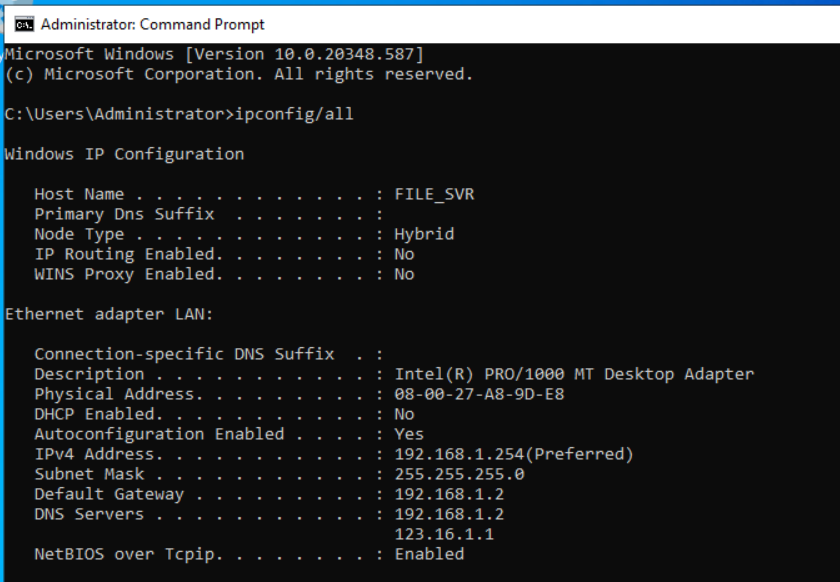
\includegraphics[width=0.7\linewidth]{SiteToSiteImg/ipFILESVR.png}
        \caption{Cấu hình IP cho máy FILE\_SVR}
    \end{figure}
    
      \item Tắt tường lửa của máy, để có thể kiểm tra đường truyền của các máy với nhau.

        \begin{figure}[htbp]
        \centering
        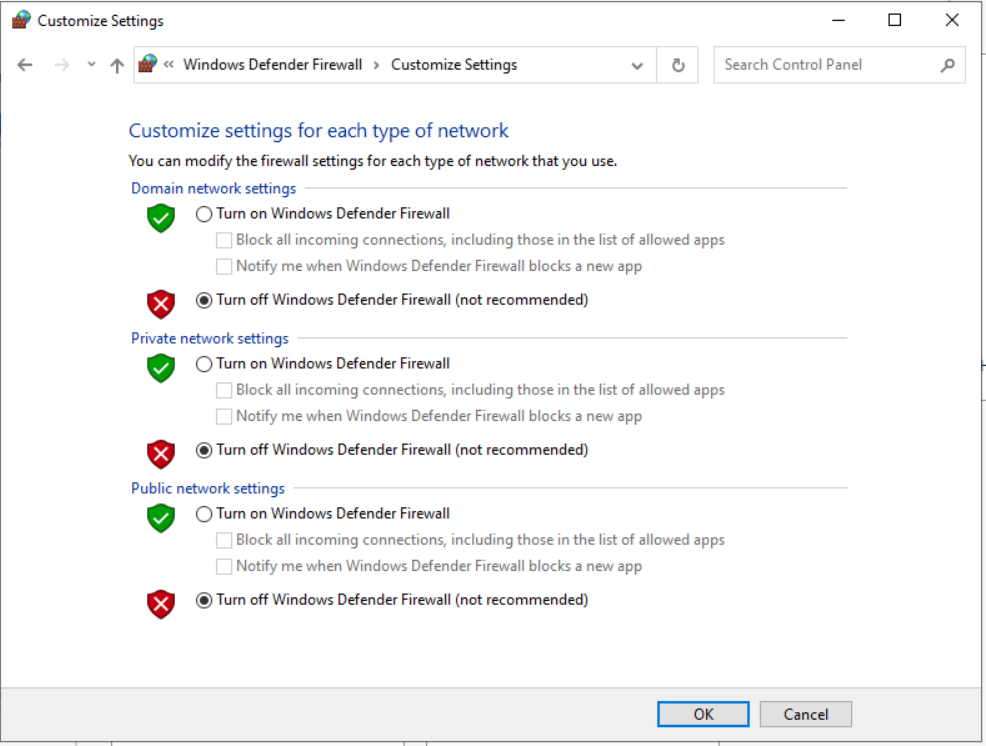
\includegraphics[width=0.5\linewidth]{SiteToSiteImg/offFirewall.png}
        \caption{Tắt firewall FILE\_SVR}
        \end{figure}
      
  \end{itemize}
    \newpage
  \textbf{\textit{Thực hiện việc cấu hình tại máy trạm Client:}}

  \begin{itemize}
      \item Cài đặt địa chỉ IP cho máy Client.
      
      \begin{figure}[htbp]
        \centering
        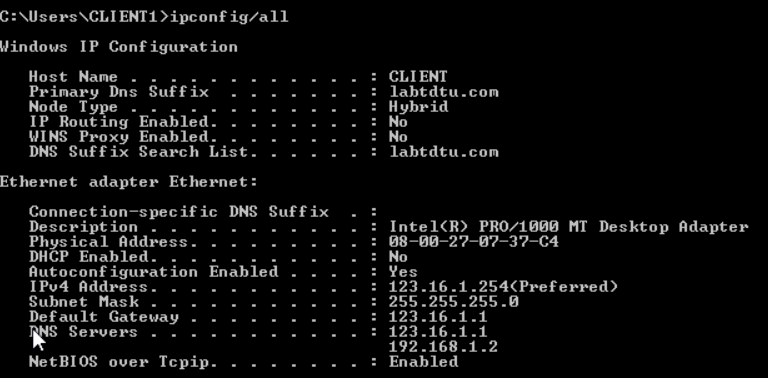
\includegraphics[width=0.5\linewidth]{SiteToSiteImg/ipClient.png}
        \caption{Cấu hình IP cho máy Client}
    \end{figure}
    
      \item Tắt tường lửa của máy như FILE\_SVR, để có thể kiểm tra đường truyền của các máy với nhau.

       \begin{figure}[htbp]
        \centering
        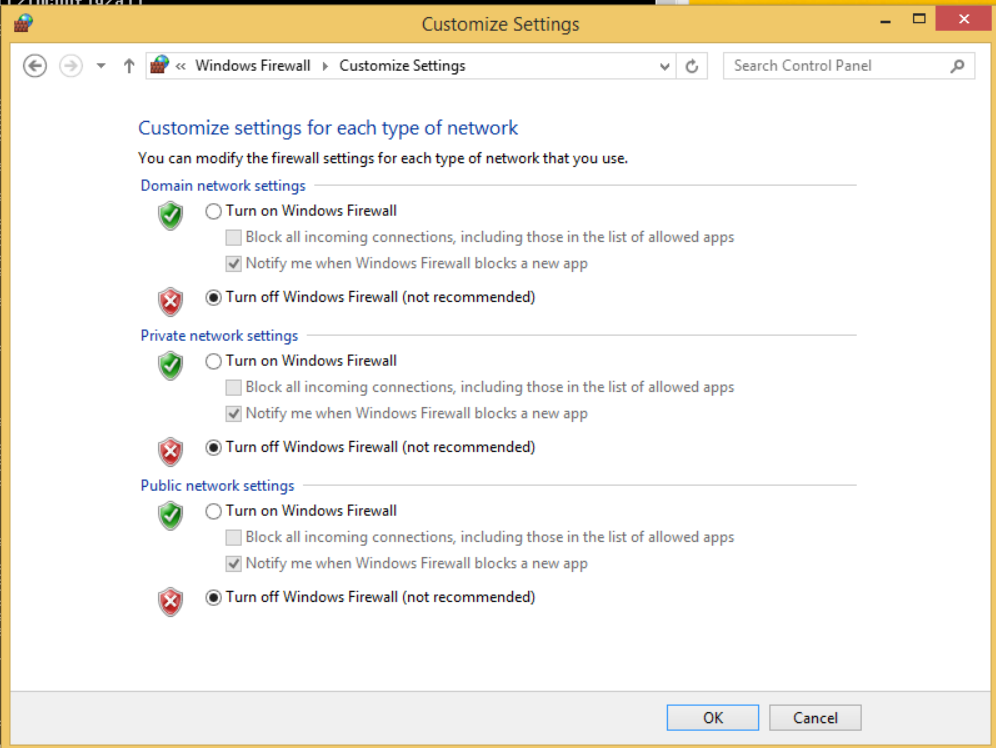
\includegraphics[width=0.4\linewidth]{SiteToSiteImg/offFirewallClient.png}
        \caption{Tắt firewall Client}
        \end{figure}
  \end{itemize}
\newpage
  \textbf{\textit{Thực hiện cấu hình tại máy TPHCM\_SVR:}}
   \begin{itemize}
      \item Máy TPHCM\_SVR được cài network có 2 card mạng, sau đó đặt tên cho từng mạng lần lượt là LAN, WAN.
       \begin{figure}[htbp]
        \centering
        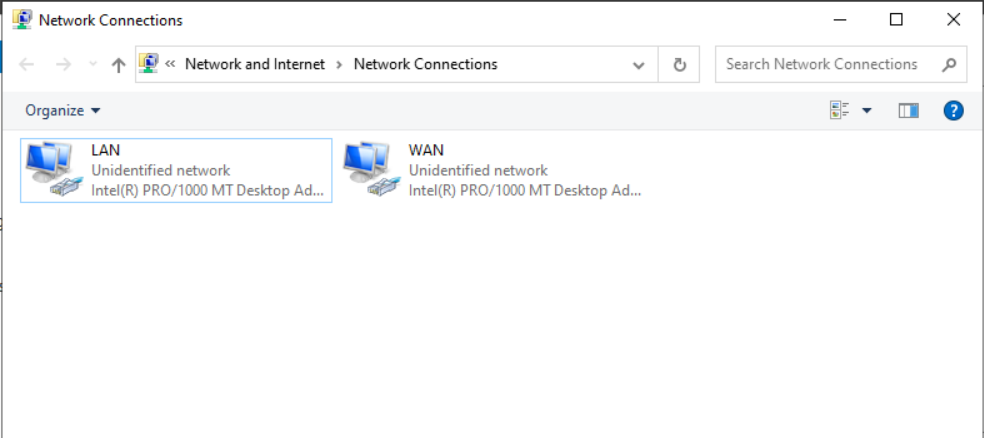
\includegraphics[width=0.5\linewidth]{SiteToSiteImg/cardNetwork.png}
        \caption{Tạo 2 card mạng cho máy VPN Server}
        \end{figure}
      \item Cài đặt địa chỉ IP cho từng card mạng của máy TPHCM\_SVR theo bảng IP:
      
        \begin{figure}[htbp]
        \centering
        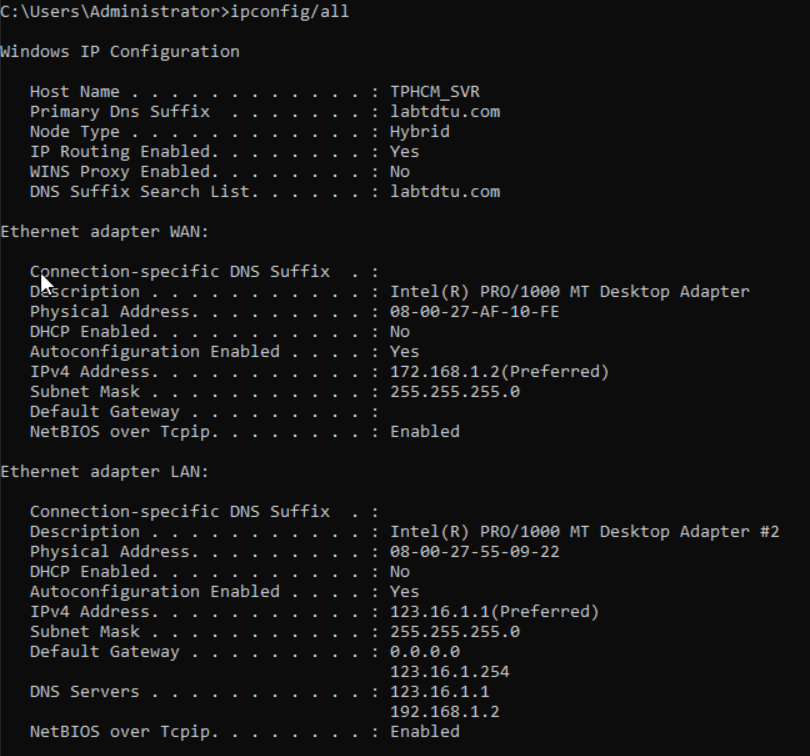
\includegraphics[width=0.5\linewidth]{SiteToSiteImg/ipHCM.png}
        \caption{Cấu hình IP cho card mạng LAN và WAN}
        \end{figure}
        
      \item Tắt tường lửa của máy, tiến hành gửi gói tin để kiểm tra đã kết nối đến máy trạm thành công.
\newpage
        \begin{figure}[htbp]
            \subfloat[Tắt tường lửa]
            {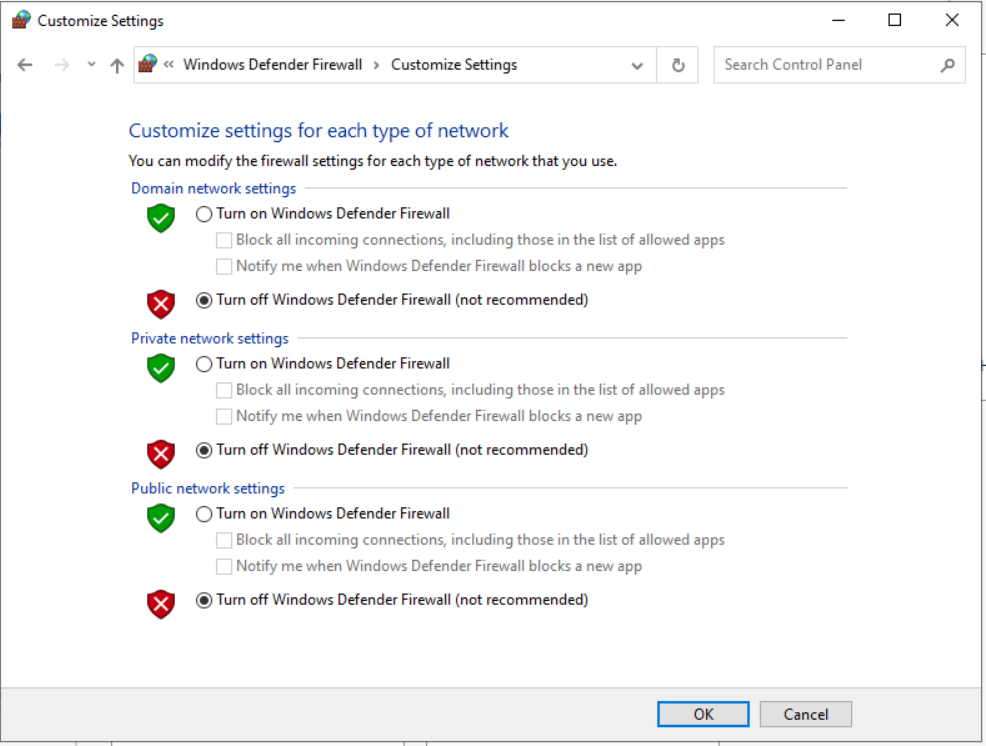
\includegraphics[width=7cm]{SiteToSiteImg/offFirewall.png}}\hfill
            \subfloat[Ping đến máy Client để kiểm tra]
            {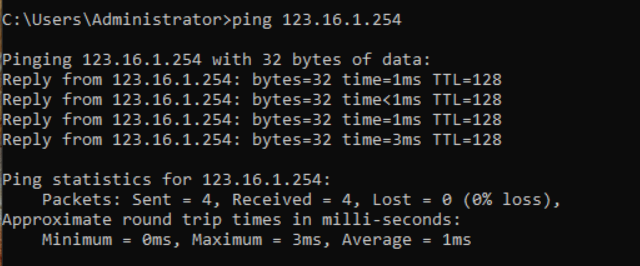
\includegraphics[width=7cm]{SiteToSiteImg/HCMpingtoClient.png}}\hfill
            \caption{Thực hiện kiểm tra đường truyền mạng của TPHCM\_SVR}
        \end{figure}
        
      \item Cài đặt Active Directory Domain Services để thiết lập miền cho chi nhánh TP.Hồ Chí Minh. Domain của máy TPHCM\_SVR là labtdtu.com, sau đó tiền hành thêm máy Client vào domain để quản lý các tài khoản người dùng nội bộ.

      \begin{figure}[htbp]
        \centering
        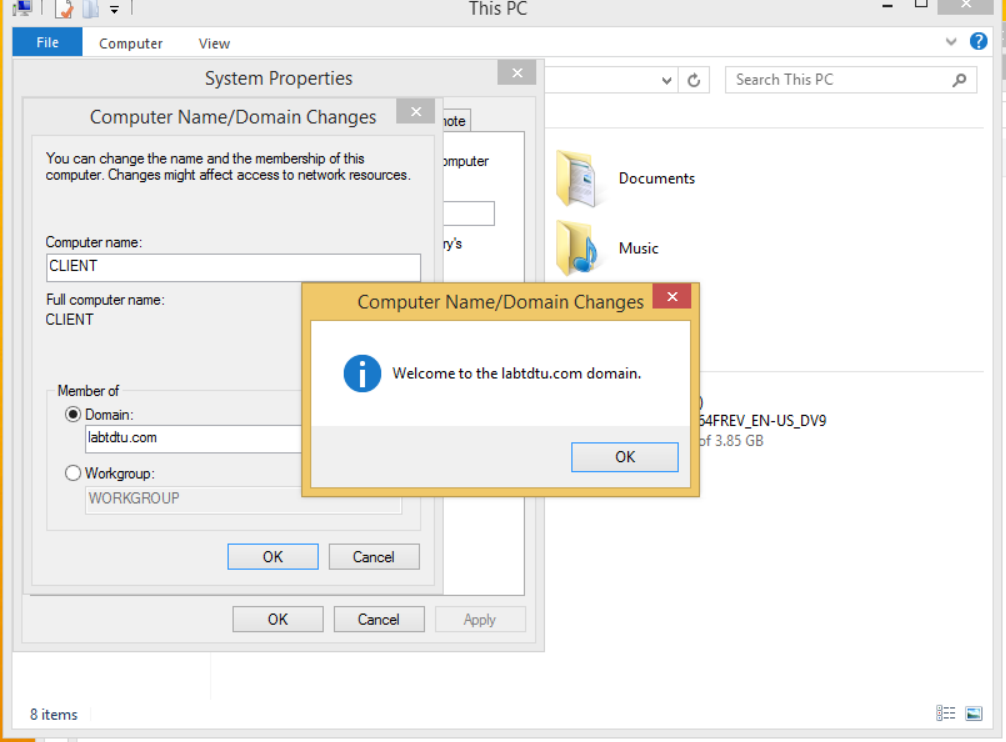
\includegraphics[width=0.7\linewidth]{SiteToSiteImg/joinClient.png}
        \caption{Thêm client vào Domain Controller}
        \end{figure}
  \end{itemize}

  \textbf{\textit{Thực hiện cấu hình tại máy HN\_SVR:}}
  \begin{itemize}
      \item Máy HN\_SVR cấu hình tương tự như máy TPHCM\_SVR, chỉ khác địa chỉ IP.  Tuy nhiên, domain của chi nhánh Hà Nội là labhn.com, đồng nghĩa như triển khai VPN từ chi nhánh đến chi nhánh khác hoặc từ công ty mình đến công ty đối tác.

        \begin{figure}[htbp]
            \subfloat[Cấu hình IP]
            {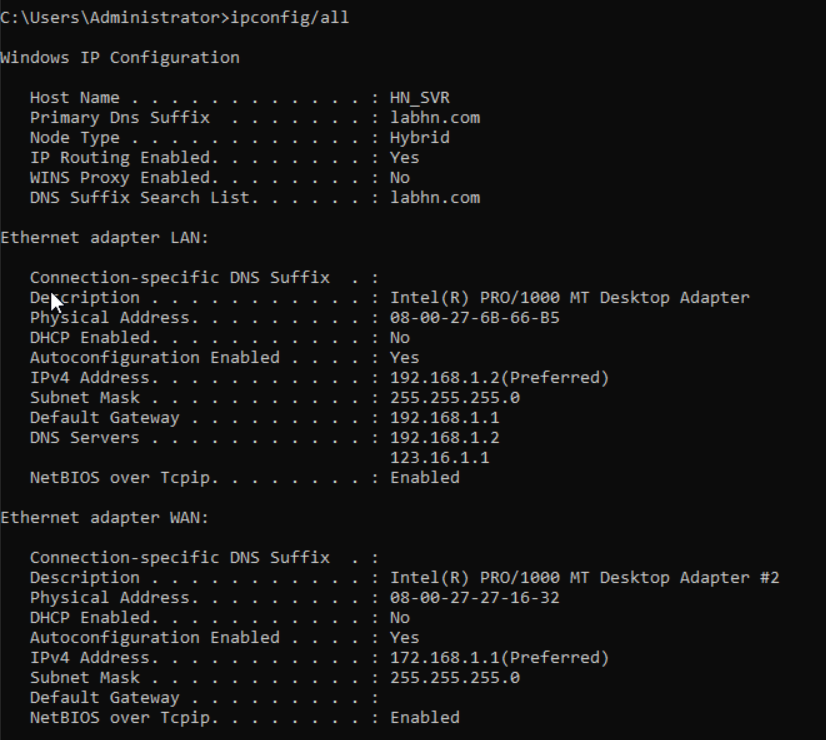
\includegraphics[width=7cm]{SiteToSiteImg/ipHNSVR.png}}\hfill
            \subfloat[Ping đến máy FILE\_SVR để kiểm tra]
            {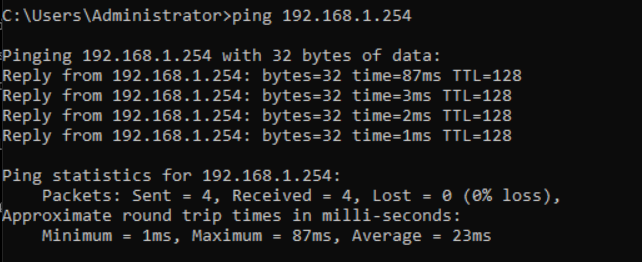
\includegraphics[width=7cm]{SiteToSiteImg/HNpingtoFILE.png}}\hfill
            \caption{Cấu hình IP và domain của HN\_SVR}
        \end{figure}

  \end{itemize}
  \textbf{\textit{Tiến hành cấu hình VPN cho 2 máy HN\_SVR và TPHCM\_SVR:}} Cả 2 máy VPN Server đều thực hiện các bước tương tự nhau.
    \begin{itemize}
        \item Chọn \textit{Add roles and features} để cài đặt Remote Access 

        \begin{figure}[htbp]
        \centering
        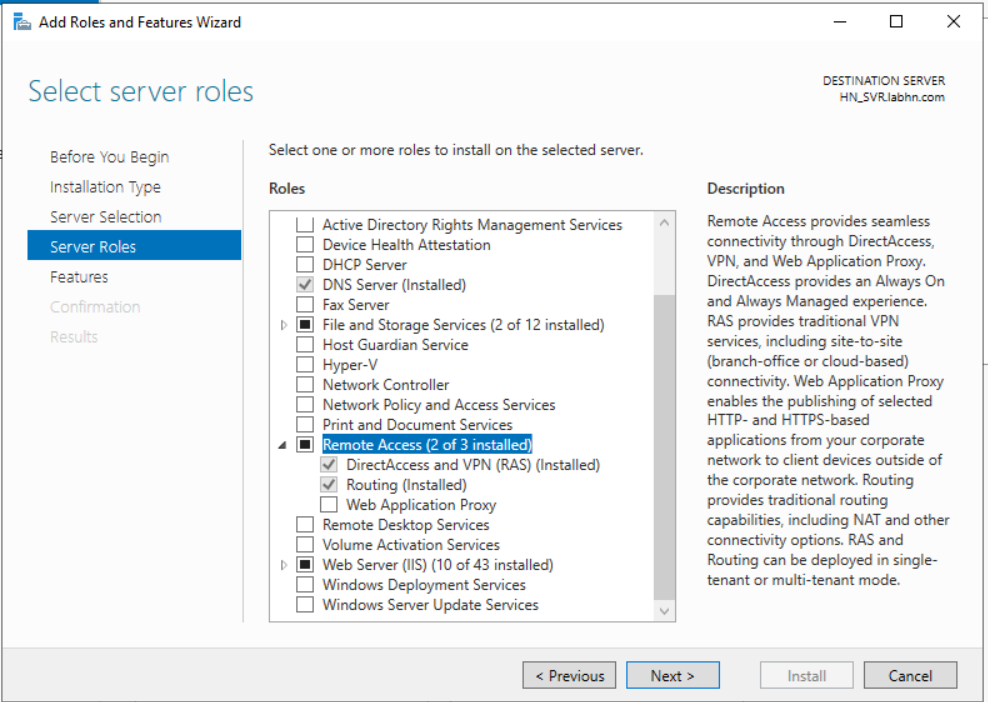
\includegraphics[width=0.7\linewidth]{SiteToSiteImg/installRemoteAccess.png}
        \caption{Cài đặt Remote Access}
        \end{figure}
        \item Trong khi chờ đợi tải Remote Access thì tạo mỗi chi nhánh một user mới, tại máy HN\_SVR tạo tài khoản có username là userhanoi và  tại máy TPHCM\_SVR tạo tài khoản có username là usersaigon. 
\newpage
        \begin{figure}[htbp]
            \subfloat[Tạo user mới ở chi nhánh Hà Nội]
            {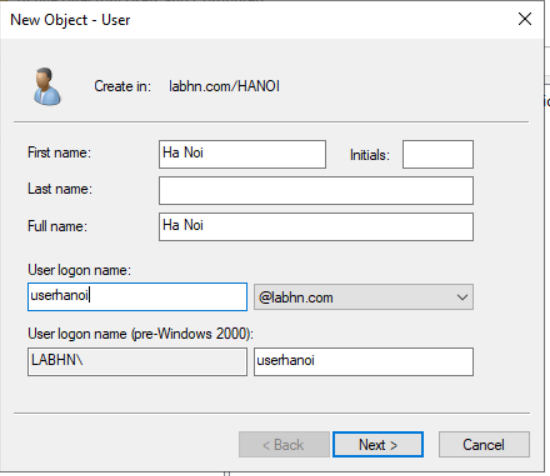
\includegraphics[width=7cm]{SiteToSiteImg/createAccHN.png}}\hfill
            \subfloat[Tạo user mới ở chi nhánh TP.HCM]
            {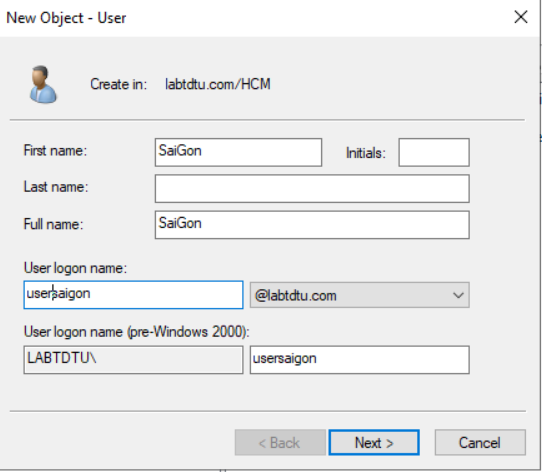
\includegraphics[width=7cm]{SiteToSiteImg/createAccSG.png}}\hfill
            \caption{Tạo user}
        \end{figure}
        \item Sau khi hoàn thành tạo user mới, click phải chọn Properties -> Dial-in -> Allow Access, cho phép tài khoản có thể truy cập vào VPN.
        
        \begin{figure}[htbp]
            \subfloat[Cài đặt user Ha Noi]
            {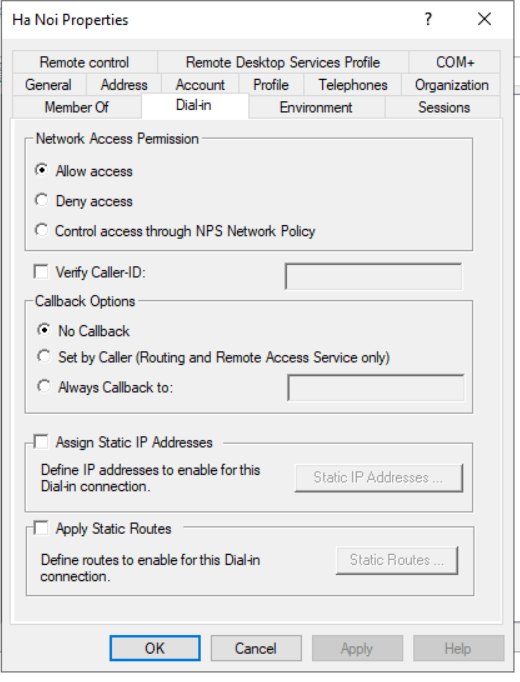
\includegraphics[width=6cm]{SiteToSiteImg/propertiesUserHN.png}}\hfill
            \subfloat[Cài đặt user SaiGon]
            {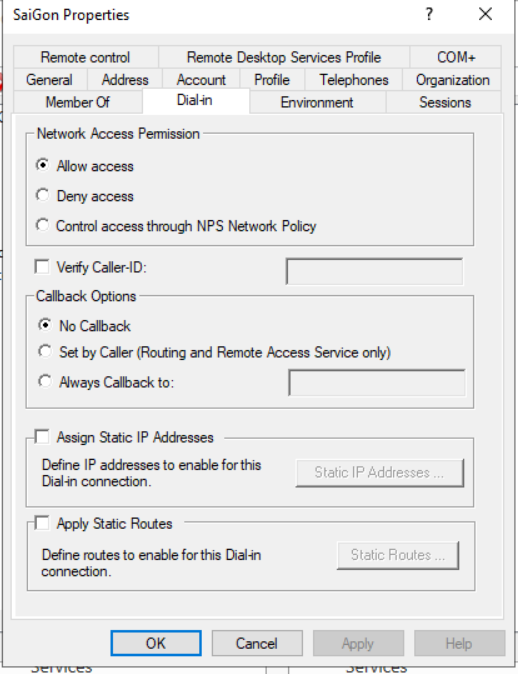
\includegraphics[width=6cm]{SiteToSiteImg/propertiesUserHCM.png}}\hfill
            \caption{Cài đặt user}
        \end{figure}
 
        \item Tại Server Manager -> Tools -> Chọn Routing and Remote Access -> click phải ở server -> chọn Configure and Enable Routing and Remote Access. Chọn Next -> Custom configuration -> Click vào 3 services như hình -> Next -> Finish -> Start Services.
        \begin{figure}[htbp]
            \subfloat[Custom Configuration]
            {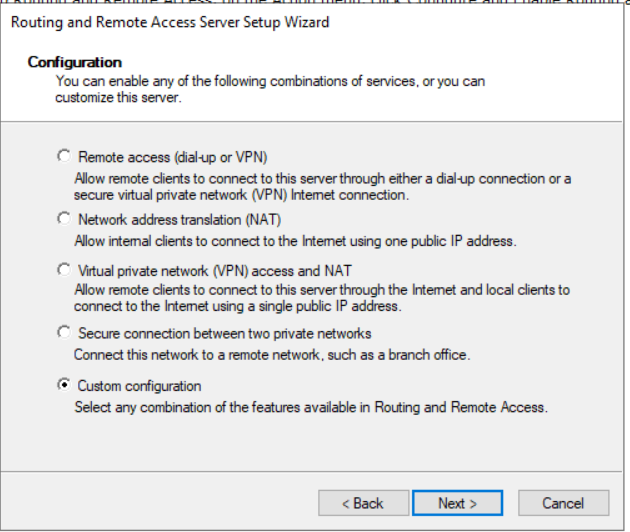
\includegraphics[width=7cm]{SiteToSiteImg/conf1.png}}\hfill
            \subfloat[Chọn services]
            {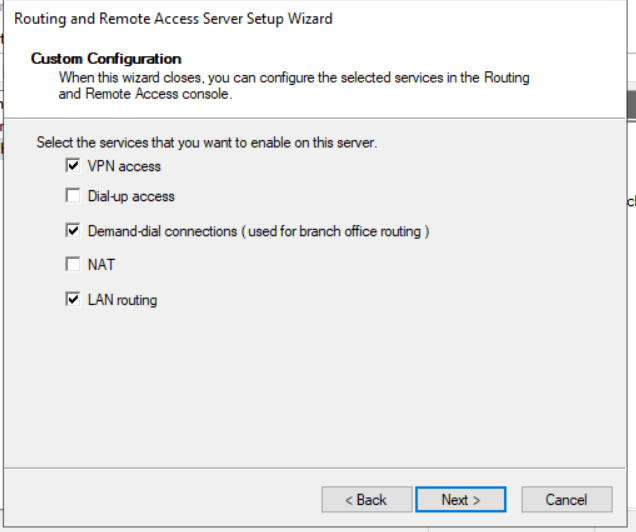
\includegraphics[width=7cm]{SiteToSiteImg/conf2.png}}\hfill
            \caption{Cấu hình và kích hoạt dịch vụ Remote Access}
        \end{figure}
        \newpage
        \item Tiếp tục click phải ở server -> Chọn Properties -> Tab Security -> Chọn Allow custom IPSec -> Nhập Key -> Chọn Tab IPv4, nhập dãy IP để cấp phát cho VPN. 

            \begin{figure}[htbp]
            \centering
            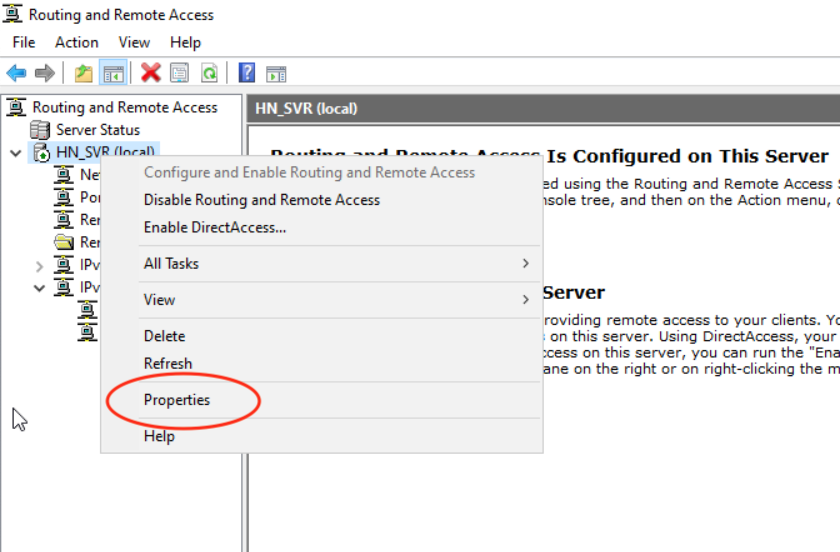
\includegraphics[width=0.7\linewidth]{SiteToSiteImg/conf3.png}
            \caption{Properties}
            \end{figure}
        
            \begin{figure}[h]
            \subfloat[Chọn IPSec và nhập Key]
            {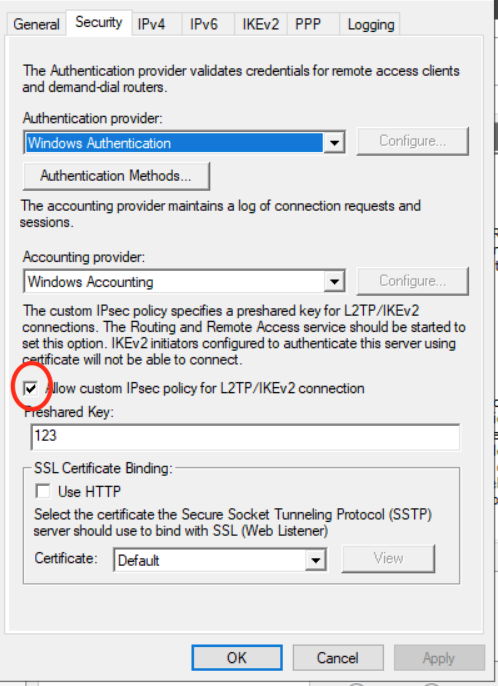
\includegraphics[width=6cm]{SiteToSiteImg/conf4.png}}\hfill
            \subfloat[Cài dãy IP cấp phát]
            {\includegraphics[width=6cm]{SiteToSiteImg/conf5.png}}\hfill
            \caption{Cài đặt dịch vụ}
        \end{figure}
        \newpage
        \item Click phải Network Interfaces -> New Demand-dial interface, để tạo VPN kết nối với chi nhánh còn lại. Tại máy TPHCM\_SVR đặt tên VPN\_HN, ngược lại tại máy HN\_SVR đặt tên là VPN\_HCM.
        \begin{figure}[htbp]
            \subfloat[New Demand-dial]
            {\includegraphics[width=7cm]{SiteToSiteImg/conf6.png}}\hfill
            \subfloat[Đặt tên VPN]
            {\includegraphics[width=7cm]{SiteToSiteImg/conf7_VPNnameHCM.png}}\hfill
            \caption{Tạo VPN}
        \end{figure}
        \item Tiếp tục chọn Next -> Chọn giao thức mong muốn, Next.
\newpage
            \begin{figure}[htbp]
            \centering
            \includegraphics[width=0.6\linewidth]{SiteToSiteImg/conf8.png}
            \caption{Chọn giao thức}
            \end{figure}
        
        \item Khi hoàn tất việc chọn giao thức, tại máy TPHCM\_SVR nhập IP WAN của HN\_SVR, ngược lại tại máy HN\_SVR nhập IP WAN của TPHCM\_SVR. Chọn Next.
        
    \end{itemize}
     \begin{figure}[htbp]
            \subfloat[Tại máy TPHCM\_SVR]
            {\includegraphics[width=7cm]{SiteToSiteImg/conf12_callIPHN.png}}\hfill
            \subfloat[Tại máy HN\_SVR]
            {\includegraphics[width=7cm]{SiteToSiteImg/conf9_callIPWANHCM.png}}\hfill
            \caption{Gọi đến IP WAN của từng máy}
        \end{figure}
    \begin{itemize}

        \item Cấu hình phần services như ảnh, chọn Next.
        \newpage
        \begin{figure}[htbp]
            \centering
            \includegraphics[width=0.6\linewidth]{SiteToSiteImg/conf9_afterCall.png}
            \caption{Chọn dịch vụ}
            \end{figure}
        \item Tại màn hình tiếp sẽ nhập đường mạng LAN của từng chi nhánh. Chi nhánh Hà Nội có đường mạng là 192.168.1.0/24 và chi nhánh TP.Hồ Chí Minh có đường mạng là 123.16.1.0/24. Nhập bước nhảy là 1 -> OK -> Chọn Next.
        
    \end{itemize}
        \begin{figure}[htbp]
            \subfloat[Tại máy TPHCM\_SVR]
            {\includegraphics[width=7cm]{SiteToSiteImg/conf13_10.png}}\hfill
            \subfloat[Tại máy HN\_SVR]
            {\includegraphics[width=7cm]{SiteToSiteImg/conf10_13.png}}\hfill
            \caption{Thiết lập lớp mạng}
    \end{figure}
    \begin{itemize}
        \item Nhập tài khoản user đã nhập từ đầu vào VPN, cho phép user có thể kết nối đến VPN. Chọn Next, hoàn tất việc tạo VPN.
        \begin{figure}[htbp]
            \subfloat[Tại máy TPHCM\_SVR]
            {\includegraphics[width=6cm]{SiteToSiteImg/conf11_14.png}}\hfill
            \subfloat[Tại máy HN\_SVR]
            {\includegraphics[width=6cm]{SiteToSiteImg/conf14_11.png}}\hfill
            \caption{Nhập user vào VPN}
        \end{figure}
        \newpage
        \item Chọn vào VPN vừa tạo, click phải chọn Properties -> Security -> Đảm bảo VPN đang ở giao thức L2TP/IPSec -> Advanced Settings -> Click Use preshared... -> Nhập key 123 như đã cài vào VPN.
        


    \begin{figure}[htbp]
            \subfloat[Chọn Properties]
            {\includegraphics[width=6cm]{SiteToSiteImg/conf15.png}}\hfill
            \subfloat[Nhập key]
            {\includegraphics[width=5cm]{SiteToSiteImg/conf16.png}}\hfill
            \caption{Cấu hình VPN vừa tạo}
        \end{figure}
  
        \item Khi hoàn thành các cấu hình thì click phải VPN của cả 2 máy chọn Connect, để kết nối với nhau. 

    \end{itemize}
 \subsubsection*{4.1.2.4 Thực nghiệm}
 \addcontentsline{toc}{subsubsection}{4.1.2.4 Thực nghiệm}
Trước khi 2 VPN kết nối với nhau, kiểm tra kết quả trả về của máy Client gọi tới máy FILE\_SVR. Kết quả không thể truy cập vào FILE\_SVR.
\newpage
    \begin{figure}[htbp]
        \centering
        \includegraphics[width=0.5\linewidth]{SiteToSiteImg/beforeConnect.png}
        \caption{Kiểm tra trước khi kết nối VPN}
    \end{figure}
    
  Sau khi triển khai, cấu hình VPN và kết nối 2 máy Server. Máy Client thực hiện lại việc liên lạc đến máy FILE\_SVR. Kết quả máy Client có thể truy cập vào FILE\_SVR và sử dụng được các tài liệu, máy in được chia sẽ trên đường mạng.

    \begin{figure}[htbp]
            \subfloat[Ping đến FILE\_SVR ]
            {\includegraphics[width=7cm]{SiteToSiteImg/afterConnect.png}}\hfill
            \subfloat[Truy cập được tài liệu, máy in được chia sẻ]
            {\includegraphics[width=7cm]{SiteToSiteImg/userData.png}}\hfill
            \caption{Kết quả sau khi kết nối VPN}
        \end{figure}
 \section*{4.2 Triển khai VPN trên Windows Server (CORE)}
 \addcontentsline{toc}{section}{4.2 Triển khai VPN trên Windows Server (CORE)}


 \subsection*{4.2.1 Xây dựng Remote Access VPN}
 \addcontentsline{toc}{subsection}{4.1.1 Xây dựng Remote Access VPN}
 \subsubsection*{4.2.1.1 Chuẩn bị thiết bị}
 \addcontentsline{toc}{subsubsection}{4.2.1.1 Chuẩn bị thiết bị}

  \begin{itemize}
     \item Một máy chủ SERVER làm VPN Server.
     \item Một máy CLIENT làm người dùng client ở ngoài Internet có thể truy cập vào mạng doanh nghiệp để lấy tài liệu làm việc.
 \end{itemize}

 \subsubsection*{4.2.1.2 Thực hiện cấu hình}
 \addcontentsline{toc}{subsubsection}{4.2.1.2 Thực hiện cấu hình}
 Tại phần cấu hình bằng phiên bản CORE, VPN sẽ được cấu hình bằng giao thức L2TP/IPSec.
 
\textbf{\textit{Thực hiện lệnh cấu hình tại máy SERVER:}}
\begin{itemize}
    \item Sử dụng lệnh cấu hình địa chỉ IP và tắt Firewall của máy:

    \begin{figure}[htbp]
        \centering
        \includegraphics[width=0.5\linewidth]{coreRemoteAccess/setIPv4.png}
        \caption{Set địa chỉ IP}
    \end{figure}
    \begin{figure}[htbp]
        \centering
        \includegraphics[width=0.5\linewidth]{coreRemoteAccess/TatTuongLuaServer.png}
        \caption{Tắt Firewall}
    \end{figure}

    \item Cài đặt các vai trò Remote Access:
    \begin{figure}[htbp]
            \subfloat[ ]
            {\includegraphics[width=7cm]{coreRemoteAccess/vaitro.png}}\hfill
            \subfloat[]
            {\includegraphics[width=7cm]{coreRemoteAccess/vaitro (2).png}}\hfill
            \caption{Cài đặt vai trò của Remote Access}
        \end{figure}

    \item Cấu hình giao thức L2TP/IPsec: 
    \textit{Để cấu hình giao thức L2TP/IPSec ta thực hiện theo các bước sau: Server Manage > Tools > Routing and Remote Access.}
    
    \textit{Tiếp theo, ta nhấn chuột phải vào tên máy chủ > Properties > Security > Authentication provider > Windows Authentication}

    \textit{Cuối cùng là nhập Pre-Shared Key}
    \begin{figure}[htbp]
        \centering
        \includegraphics[width=0.5\linewidth]{coreRemoteAccess/key-l2tp.png}
        \caption{Cấu hình giao thức L2TP/IPsec}
    \end{figure}
    \newpage
    
    \item Thiết lập một dải IP cho VPN Client
    \begin{figure}[htbp]
        \centering
        \includegraphics[width=0.5\linewidth]{coreRemoteAccess/setIPClient.png}
        \caption{Thiết lập dải IP tĩnh}
    \end{figure}
    

    \item Tiến hành mở các cổng cần thiết trên Firewall
    \begin{figure}[htbp]
        \centering
        \includegraphics[width=0.5\linewidth]{coreRemoteAccess/openPort1.png}
        \caption{Mở cổng Firewall UDP 500}
        \vspace{2em}
        \includegraphics[width=0.5\linewidth]{coreRemoteAccess/openPort2.png}
        \caption{Mở cổng Firewall UDP 4500}
    \end{figure}
    
    \newpage

    \item Tạo nhóm người dùng OU và người dùng mới tại máy Server
    \begin{figure}[htbp]
        \centering
        \includegraphics[width=0.5\linewidth]{coreRemoteAccess/createOU.png}
        \caption{Tạo OU và User}
    \end{figure}

    \item Tạo thư mục "Text" tại ổ đĩa C của máy, trong thư mục đó có chứa tệp tin "XinChao.tex"
    \begin{figure}[htbp]
        \centering
        \includegraphics[width=0.5\linewidth]{coreRemoteAccess/createFile.png}
        \caption{Tạo thư mục và tệp tin}
    \end{figure}

    \item Tiến hành chia sẻ quyền truy cập của tệp tin vừa tạo
    \begin{figure}[htbp]
        \centering
        \includegraphics[width=0.5\linewidth]{coreRemoteAccess/sharefile.png}
        \caption{Chia sẻ quyền truy cập tệp tin}
    \end{figure}
    
\end{itemize}

\textbf{\textit{Thực hiện lệnh cấu hình tại máy CLIENT:}}
\begin{itemize}
    \item Sử dụng lệnh cấu hình địa chỉ IP và tắt Firewall của máy:

    \begin{figure}[htbp]
        \centering
        \includegraphics[width=0.5\linewidth]{coreRemoteAccess/setIPv4_CLient.png}
        \caption{Set địa chỉ IP}
    \end{figure}
    \begin{figure}[htbp]
        \centering
        \includegraphics[width=0.5\linewidth]{coreRemoteAccess/TatTuongLuaClient.png}
        \caption{Tắt Firewall}
    \end{figure}

    \newpage
    \item Sau khi ping thành công tới máy SERVER, ta tiến hành tạo kết nối VPN với máy SERVER.
    \begin{figure}[htbp]
        \centering
        \includegraphics[width=0.5\linewidth]{coreRemoteAccess/createVPNconnect.png}
        \caption{Tạo kết nối VPN}
    \end{figure}

    \item Tiến hành cài đặt giao thức L2TP/IPSec tại máy CLIENT như hình bên dưới và nhập mã Presharekey.
    
    \textit{Truy cập Network Connection > Nhấn chuột phải vào "VPNConnection" > Properties > Security}
    \begin{figure}[htbp]
        \centering
        \includegraphics[width=0.5\linewidth]{coreRemoteAccess/setKey.png}
        \caption{Cài đặt L2TP/IPSec tại máy CLIENT}
    \end{figure}
    \newpage
    \textit{Truy cập Network Connection > Nhấn chuột phải vào "VPNConnection" > Properties > Security > Advanced Setting > Nhập mã Presharekey > Ok.}
    \begin{figure}[htbp]
        \centering
        \includegraphics[width=0.5\linewidth]{coreRemoteAccess/setL2TP.png}
        \caption{Nhập mã Presharekey}
    \end{figure}

    \newpage
\end{itemize}

 \subsubsection*{4.2.1.3 Thực nghiệm}
 \addcontentsline{toc}{subsubsection}{4.2.1.3 Thực nghiệm}
\begin{itemize}
    \item Đầu tiên, ta sẽ join vào VPN đã được tạo
    \begin{figure}[htbp]
            \subfloat[]
            {\includegraphics[width=7cm]{coreRemoteAccess/joinVPN.png}}\hfill
            \subfloat[]
            {\includegraphics[width=7cm]{coreRemoteAccess/connecting.png}}\hfill
            \caption{Tiến hành Join vào VPN}
        \end{figure}
    \item Khi đã kết nối thành công vào VPN, tiến hành tìm kiếm tệp tin được chia sẻ và truy cập vào nó.
    \begin{figure}[htbp]
            \subfloat[Tìm kiếm tệp tin]
            {\includegraphics[width=7cm]{coreRemoteAccess/findFile.png}}\hfill
            \subfloat[Truy cập thành công]
            {\includegraphics[width=7cm]{coreRemoteAccess/Connect_ThanhCong.png}}\hfill
            \caption{Truy cập vào tệp tin được chia sẻ thành công}
        \end{figure}
    \newpage
\end{itemize}


 \subsection*{4.2.2 Xây dựng Site-to-Site VPN}
 \addcontentsline{toc}{subsection}{4.1.2 Xây dựng Site-to-Site VPN}

\subsubsection*{4.2.2.1 Chuẩn bị thiết bị}
 \addcontentsline{toc}{subsubsection}{4.2.1.1 Chuẩn bị thiết bị}
\begin{itemize}
     \item Một máy chủ HN\_SVR để quản lý VPN Server ở Hà Nội.
     \item Một máy chủ TPHCM\_SVR để quản lý  VPN Server ở TP.Hồ Chí Minh.
     \item Một máy File Server dùng dể quản lý các tài liệu, data của chi nhánh Hà Nội.
     \item Một máy trạm ở TP.Hồ Chí Minh.
 \end{itemize}
 \subsubsection*{4.2.2.2 Thực hiện cấu hình}
 \addcontentsline{toc}{subsubsection}{4.2.2.2 Thực hiện cấu hình}
 
Tại phần cấu hình bằng phiên bản CORE, VPN sẽ được cấu hình bằng giao thức SSTP.

\textbf{\textit{Thực hiện lệnh cấu hình địa chỉ IP tại các máy:}}
\begin{itemize}
    \item Sử dụng lệnh cấu hình địa chỉ IP và tắt Firewall của máy:

    \textit{- Máy FILE SERVER}\\
     \begin{figure}[htbp]
            \centering
            \includegraphics[width=0.5\linewidth]{SiteToSiteImg/ipFILE.png}
            \caption{Lệnh cấu hình IP}
        \end{figure}
        
    \textit{- Máy Client}: Vì chỉ có thể cấu hình PowerShell bằng quyền Administrator nên tại máy Client cài đặt IP bằng GUI.
     \begin{figure}[htbp]
            \centering
            \includegraphics[width=0.5\linewidth]{SiteToSiteImg/ipClient.png}
            \caption{IP Client}
        \end{figure}
    \newpage
    \item Đối với hai máy chủ VPN thì sẽ có các lệnh cấu hình IP DNS riêng:
    \begin{figure}[htbp]
        \centering
        \includegraphics[width=0.7\linewidth]{SiteToSiteImg/ipSG.png}
        \caption{Lệnh cấu hình IP máy TPHCM\_SVR}
        \vspace{2em}
        \includegraphics[width=0.7\linewidth]{SiteToSiteImg/iphn.png}
        \caption{Lệnh cấu hình IP máy HN\_SVR}
    \end{figure}
\end{itemize}
 
\textbf{\textit{Thực hiện lệnh cấu hình cho cả hai máy chủ VPN:}} 
\begin{itemize}
    \item Cài đặt Active Directory Domain Services và thiết lập miền cho máy chủ. Nhập mật khẩu là cài đặt thành công.
   \begin{figure}[htbp]
        \centering
        \includegraphics[width=0.7\linewidth]{SiteToSiteImg/domainHCM.png}
        \caption{Cấu hình domain máy TPHCM\_SVR}
    \end{figure}
     \newpage
     \begin{figure}[htbp]
     \centering
        \includegraphics[width=0.7\linewidth]{SiteToSiteImg/domainHN.png}
        \caption{Cấu hình domain máy HN\_SVR}
    \end{figure}
    \item Cài đặt Remote Access, Routing để có thể cấu hình VPN. Sau đó kiểm tra lại các cài đặt.
    \begin{figure}[htbp]
            \subfloat[Cài đặt Remote Access]
            {\includegraphics[width=7cm]{SiteToSiteImg/InstallRemote.png}}\hfill
            \subfloat[Kiểm tra]
            {\includegraphics[width=7cm]{SiteToSiteImg/checkInstall.png}}\hfill
            \caption{Cài đặt và kiểm tra Remote Access}
        \end{figure}
        
    \item Sau khi hoàn thành tạo user mới, click phải chọn Properties -> Dial-in -> Allow Access, cho phép tài khoản có thể truy cập vào VPN.
        
        \begin{figure}[htbp]
            \subfloat[Cài đặt user Ha Noi]
            {\includegraphics[width=5cm]{SiteToSiteImg/propertiesUserHN.png}}\hfill
            \subfloat[Cài đặt user SaiGon]
            {\includegraphics[width=5cm]{SiteToSiteImg/propertiesUserHCM.png}}\hfill
            \caption{Cài đặt user}
        \end{figure}
        
    \item Để có thể kết nối VPN bằng SSTP, cần phải có chứng chỉ xác thực từ máy chủ. Do máy không có sẵn chứng nên sẽ cài đặt chứng chỉ tự kí bằng lệnh sau.
    \begin{figure}[htbp]
            \subfloat[Tạo chứng chỉ cho máy HN]
            {\includegraphics[width=7cm]{SiteToSiteImg/cerHN.png}}\hfill
            \subfloat[Tạo chứng chỉ cho máy HCM]
            {\includegraphics[width=7cm]{SiteToSiteImg/cerSG.png}}\hfill
            \caption{Tạo chứng chỉ tự kí}
        \end{figure}
    \item Tại Server Manager -> Tools -> Chọn Routing and Remote Access -> click phải ở server -> chọn Configure and Enable Routing and Remote Access. Chọn Next -> Custom configuration -> Click vào 3 services như hình -> Next -> Finish -> Start Services.
    
        \begin{figure}[htbp]
            \subfloat[Custom Configuration]
            {\includegraphics[width=6cm]{SiteToSiteImg/conf1.png}}\hfill
            \subfloat[Chọn services]
            {\includegraphics[width=6cm]{SiteToSiteImg/conf2.png}}\hfill
            \caption{Cấu hình và kích hoạt dịch vụ Remote Access}
        \end{figure}

    \item Tiếp tục click phải ở server -> Chọn Properties -> Tab Security -> Tại Certificate chọn chứng chỉ vừa mới tạo -> Click chọn Use HTTP ->  Chọn Tab IPv4, nhập dãy IP để cấp phát cho VPN -> Apply
\newpage
    \begin{figure}[htbp]
            \centering
            \includegraphics[width=0.5\linewidth]{SiteToSiteImg/conf3.png}
            \caption{Properties}
        \end{figure}
    
    \begin{figure}[htbp]
            \subfloat[Chọn User HTTP]
            {\includegraphics[width=7cm]{SiteToSiteImg/clickCer.png}}\hfill
            \subfloat[Cài dãy IP cấp phát]
            {\includegraphics[width=7cm]{SiteToSiteImg/conf5.png}}\hfill
            \caption{Cài đặt dịch vụ}
        \end{figure}
        
    \item Tiến hành tạo VPN vào interface với lệnh Add-VpnS2SInterface.
    \newpage
    \begin{figure}[htbp]
        \centering
        \includegraphics[width=0.7\linewidth]{SiteToSiteImg/creat2.png}
        \caption{Tại máy TPHCM\_SVR}
        \vspace{2em}
        \includegraphics[width=0.7\linewidth]{SiteToSiteImg/creat1.png}
        \caption{Tại máy HN\_SVR}
    \end{figure}
    
    \item Kiểm tra các VPN đã tạo trên RRAS
    \begin{figure}[htbp]
            \centering
            \includegraphics[width=0.7\linewidth]{SiteToSiteImg/check.png}
            \caption{Kiểm tra VPN đã tạo}
        \end{figure}
    \item Kết quả trả về cho thấy VPN đã được tạo, tuy nhiên vẫn chưa được định tuyến đến đường mạng của máy chủ đích. Do lệnh thêm địa chỉ định tuyến không được hỗ trợ nên thực hiện bằng cách thủ công. Chọn IPV4 -> Static Route -> Thêm địa chỉ.

    \begin{figure}[htbp]
            \centering
            \includegraphics[width=0.5\linewidth]{SiteToSiteImg/newRoute.png}
            \caption{Tạo IP định tuyến}
        \end{figure}
    \newpage
    \begin{figure}[htbp]
            \subfloat[Tại máy TPHCM\_SVR]
            {\includegraphics[width=7cm]{SiteToSiteImg/routeHN.png}}\hfill
            \subfloat[Tại máy HN\_SVR]
            {\includegraphics[width=7cm]{SiteToSiteImg/routeHCM.png}}\hfill
            \caption{Định tuyến}
        \end{figure}
    \item Start-Service lại máy chủ, chọn connect hai VPN vừa tạo
    \begin{figure}[htbp]
            \subfloat[Tại máy TPHCM\_SVR]
            {\includegraphics[width=7cm]{SiteToSiteImg/conf17.png}}\hfill
            \subfloat[Tại máy HN\_SVR]
            {\includegraphics[width=7cm]{SiteToSiteImg/conf18.png}}\hfill
            \caption{Connect VPN}
        \end{figure}
    \item Kiểm tra gửi gói tin đến IP mạng WAN của máy chủ đích.
    \begin{figure}[htbp]
            \centering
            \includegraphics[width=0.5\linewidth]{SiteToSiteImg/testping.png}
            \caption{Kiểm tra}
        \end{figure}
\end{itemize}

\newpage
 \subsubsection*{4.2.2.3 Thực nghiệm}
 \addcontentsline{toc}{subsubsection}{4.2.2.3 Thực nghiệm}

Sử dụng máy Client để ping đến hai địa chỉ máy chủ VPN của Hà Nội để kiểm tra kết quả trước khi kích hoạt VPN. Kết quả không thể gửi gói tin tới máy chủ. 

    \begin{figure}[htbp]
        \centering
        \includegraphics[width=0.5\linewidth]{SiteToSiteImg/testClient.png}
        \caption{Kiểm tra trước khi kết nối VPN}
    \end{figure}

    Sau khi triển khai, cấu hình VPN và kết nối 2 máy Server. Máy Client thực hiện lại việc liên lạc đến máy FILE\_SVR. Kết quả máy Client có thể truy cập vào FILE\_SVR và sử dụng được các tài liệu, máy in được chia sẽ trên đường mạng.

    \begin{figure}[htbp]
            \subfloat[Ping đến FILE\_SVR ]
            {\includegraphics[width=7cm]{SiteToSiteImg/afterConnect.png}}\hfill
            \subfloat[Truy cập được tài liệu, máy in được chia sẻ]
            {\includegraphics[width=7cm]{SiteToSiteImg/netview.png}}\hfill
            \caption{Kết quả sau khi kết nối VPN}
        \end{figure}